\documentclass{article}

\usepackage{amsmath}
\usepackage{amsfonts}
\usepackage{amssymb}
\usepackage{graphicx}
\usepackage{subcaption}
\usepackage[colorinlistoftodos]{todonotes}
\usepackage[colorlinks=true, allcolors=blue]{hyperref}
\usepackage[margin=1in]{geometry}

\usepackage{tikz}
\usetikzlibrary{positioning}
\usetikzlibrary{shapes,arrows}
\usepackage{adjustbox}
\tikzstyle{decision} = [diamond, draw, fill=blue!20,
        text width=4.5em, text badly centered, node distance=3cm, inner sep=0pt]
        \tikzstyle{block} = [rectangle, draw, fill=blue!20,
                text width=6em, text centered, rounded corners, minimum height=4em]
                \tikzstyle{line} = [draw, -latex']
                \tikzstyle{cloud} = [draw, ellipse,fill=red!20, node distance=3cm,
                        minimum height=2em]

\graphicspath{ {figures/} }

\usepackage{algorithm}
\usepackage[noend]{algpseudocode}

% Commands
\newcommand{\alphabet}{\mathcal{A}}

%EM Let's decide if we want to focus on generative model validation as a primary aim or as an application.
%EM One could imagine writing this either way-- the application would be "repertoires are complex. here's a bunch of summary statistics and a standard means of comparing them. one can use them to compare repertoires, be they simulated or real."
%BJO To me it seems that model validation provides a more substantive goal, but I'm willing to consider either option. Do you have a preference?
%EM I prefer having both.
\title{Immune receptor repertoire comparison and model validation via summary statistics}
\author{Branden Olson, Software WG folks, Frederick A Matsen IV}

\begin{document}

\maketitle

\begin{abstract}
The adaptive immune system generates an incredible diversity of antigen receptors to keep dangerous pathogens at bay.
    The DNA sequences coding for these receptors arise by a complex process of random naive cell generation followed by a series of binding-based filters as well as affinity maturation for B cells, giving considerable structure to the distribution of sequences.
This structure leads to Rep-Seq datasets whose analysis is difficult but important for scientific understanding and public health applications.
One can compare these data sets to each other and to generative model simulations using summary statistics, or quantities that summarize some aspect of the repertoires.
In this paper we introduce \texttt{sumrep}, an R package that performs a wide variety of repertoire summaries and comparisons, and show how \texttt{sumrep} can be used to perform model validation.
We find regarding the summary statistics...
We find regarding the models...
\end{abstract}

\section*{Introduction}

B cells and T cells play critical roles in adaptive immunity through the cooperative identification of and response to antigens.
The sophisticated rearrangement of the genes that construct B cell receptors (BCRs) and T cell receptors (TCRs) allows for the recognition of a highly diverse set of antigen epitopes.
We refer to the set of lymphocyte receptors present in an individual's immune system as their immune receptor repertoire; this repertoire constantly changes over the course of an individual's lifetime for various reasons including differences in germline gene sets and exposure to antigens.

The random generation of immune repertoires from gene rearrangements invites probabilistic modeling along with model-based simulation for generative models.
In particular, one can benchmark generative model-based inferential tools by applying them to simulations from the assumed model and assessing the tool's performance.
Simulation tools can also be used to generate a null distribution to compare to data to look for a specific effect, such as natural selection \cite{Yaari2012-kk}.

To build and improve on such probabilistic frameworks, we must identify the strengths and limitations of the underlying models.
One form of statistical model validation compares features of simulated data to observed repertoire samples and evaluates their concordance (or lack thereof).
This is not as easy a task for repertoires as it is for other problems, where a model output may simply be a real number.
In contrast, repertoire models generate sets of nucleotide sequences that are sparse in the very large set of all possible nucleotide sequences.
Moreover, the most realistic repertoire models incorporate various underlying structures such as clonal family clusters or phylogenetic trees, further compounding the difficulties.
Indeed, immune repertoires are large, complex objects.

In such a setting, summary statistics are useful (and sometimes sufficient) for expressing discrepancies between model simulations and data, and also between simulations and between data sets.
Luckily, researchers have already derived many means of quantifying important features of repertoires.
These summary statistics can range from simple statistics such as the level of GC content, to statistics such as tree shapes which are applied to complex inferences.
Simple statistics acting on raw sequences are helpful because they are robust to potentially problematic assumptions of inferential methods as well as implementation intricacies.
For example, in linear regression, comparing inferred slopes is less useful when the relationship of the data is not truly linear, but comparing nonparametric statistics like the sample mean or range is still sensible.
On the other hand, more intricate statistics give more precise descriptions of the data and can yield more elaborate insights than simple ones.
For example, model-based statistics are revealing when inferential model fit is reasonable, and can help reduce noise from sampling or measurement error.
In our linear regression example, comparing the general trends of points can be less distracted by noise than comparing the sets of points directly, and can differentiate between linear associations unlike the sample mean.

Still, determining how well a given summary can describe or distinguish a repertoire is a difficult task.
To illustrate, as noted above, a BCR repertoire can be abstracted as a collection of trees, with nucleotide sequences at the nodes.
Thus, repertoires are substantially more complex than trees, and even for the strictly simpler problem of summarizing trees, there has been a lot of effort to define good summary statistics \cite{Mooers1997-jl}.
Tree statistics, albeit other ones, have also been a major focus of previous work in BCR sequence analysis \cite{Dunn-Walters2004-hv,Mehr2004-ej,Steiman-Shimony2006-fm,Shahaf2008-cc}.
These difficulties suggest that an eclectic approach using many diverse summaries should give a thorough view of a repertoire's characteristics.

[Cartoon of projecting repertoires in various directions into real space, and comparing the resulting projections?]

In this paper, we gather dozens of meaningful summary statistics on repertoires, derive efficient and robust summary implementations, and identify appropriate comparison methods for each summary.
We present \texttt{sumrep}, an R package that computes these summary distributions for Rep-Seq datasets and performs repertoire comparisons based on these summaries.
We show how \texttt{sumrep} can be used for model validation through case studies of two state-of-the-art repertoire simulation tools: \texttt{partis} \cite{Ralph2016-nw, Ralph2016-iz} for BCRs and \texttt{IGoR} \cite{Marcou2018-du} for TCRs.
Furthermore, we investigate the effectiveness of various summary statistics in distinguishing between different observed repertoires as well as between simulated and observed data.
%BJO - Not sure what is meant by the below line.
Although by comparing various generative models to real data, we obtain a validated means of generating data for benchmarking inferential tools, we don't do that here.
Also, although summary statistics can be used in simulation-based inferential methods such as approximate Bayesian computation, we don't do that here either.

\subsection*{Repertoire Comparison}

%EM This next paragraph doesn't feel abstract methods-y.
%BJO It may eventually be a better fit for a Discussion section, but I'll put it here for now.
Applications of a methodical lymphocyte repertoire comparison tool include:
\begin{itemize}
\item Comparing simulated repertoires to observed ones, such as for model selection and validation
\item Contrasting repertoires in the context of antigen response or vaccination design and evaluation
\item Assessing the performance of competing repertoire analysis tools
\item Evaluating artificial lymphocyte repertoires \cite{Finlay2012}
\end{itemize}

\section*{Methods}

\begin{table}
\makebox[\textwidth][c]{ % this centers a too-wide table
\begin{tabular}{c|c|c|c|c}
    Summary statistic & Annotations & Clustering & Phylogeny & Implementation
\\
\hline \hline
    Pairwise distance distribution & No & No & No & \texttt{stringdist} \cite{vanderLoo2014-re} \\
$k$th nearest neighbor distribution & No & No & No & \texttt{stringdist} \\
    GC-content distribution & No & No & No & \texttt{ape} \cite{Paradis04-hz} \\
    Hot/cold spot motif count distribution & No & No & No & \texttt{Biostrings} \cite{Pagès17-bi} \\
\hline
Distance from naive to mature distribution & Yes & No & No & \texttt{stringdist} \\
%BJO Another one we kind of skipped over.
$k$th nearest neighbor (V-sequence) distribution & Yes & No & No &\texttt{stringdist},  \texttt{sumrep} \\
CDR3 length distribution & Yes & No & No & Tool-provided \\
Joint distribution of germline gene use & Yes & No & No & \texttt{sumrep} \\
Pairwise CDR3 distance distribution & Yes & No & No & \texttt{stringdist} \\
    Hydrophobicity distribution & Yes & No & No & \texttt{Peptides} \cite{Osorio15-tv} \\
    Atchley factors distribution & Yes & No & No & \texttt{HDMD} \cite{McFerrin13-ng} \\
Aliphatic index distribution & Yes & No & No & \texttt{Peptides} \\
    G.R.A.V.Y. index distribution & Yes & No & No & \texttt{alakazam} \cite{Gupta2015-iu} \\
Per-gene substitution rate & Yes & No & No & Tool-provided + \texttt{sumrep} \\
Per-gene-per-position substitution rate & Yes & No & No & Tool-provided + \texttt{sumrep} \\
Per-base mutability model & Yes & No & No & \texttt{shazam} \cite{Gupta2015-iu} \\
Per-base substitution model & Yes & No & No & \texttt{shazam} \\
%BJO This one doesn't depend on fit-star, right?
%EM Yes, but we could just count Ts vs Tv, call it a "ratio" and drop the model-based rigor.
Transition/transversion ratio distribution & Yes & No & No & \texttt{sumrep} \\
Positional distance between mutations distribution & Yes & No & No & \texttt{sumrep}  \\
Distance from naive to mature distribution & Yes & No & No & \texttt{stringdist} \\
V/D/J deletion/insertion lengths distribution & Yes & No & No & Tool-provided \\
Transition matrix for insertions & Yes & No & No & \texttt{sumrep} \\
\hline
Cluster size distribution & Yes & Yes & No & Custom \\
Hill numbers (diversity indices) & Yes & Yes & No & \texttt{alakazam} \\
Selection estimates & Yes & Yes & No & \texttt{shazam} \\
%BJO blocked due to fit-star
Transition/transversion rates & Yes & Yes & No & Tool-provided \\
\hline
    Sackin index distribution & Yes & Yes & Yes & \texttt{CollessLike} \cite{Mir2018-lk} \\
Colless-like index distribution & Yes & Yes & Yes & \texttt{CollessLike} \\
Cophenetic index distribution & Yes & Yes & Yes & \texttt{CollessLike} \\
%BJO To be delineated
Graph-theoretical features & Yes & Yes & Yes & TBD \\
\end{tabular}
}
\caption{Working table of summary statistics as well as their respective levels of assumed post-processing.}
\label{tab:SummaryStatistics}
\end{table}

Table \ref{tab:SummaryStatistics} lists the summary statistics currently supported by \texttt{sumrep}, and includes the assumed level of annotation, clustering, and phylogenetic inference.
The first group does not require any post-processing and are completely tool-independent.
The second group requires standard sequence annotations, such as inferred naive ancestor sequences, germline gene assignments, and indel information.
The third group also requires clonal family cluster assignments.
The fourth group further requires an imputed phylogeny for each clonal family.
\texttt{sumrep} itself does not perform any annotation, clustering, or phylogeny inference, but rather assumes such metadata have been pre-computed and included in the given dataset; in principle, one can use any tool which performs these tasks as expected.

Other possible statistics:

\begin{itemize}
\item Clustered sequences: estimated total diversity reviewed in \cite{Mehr2012-se}
\item Trees: graph theoretical features \cite{Dunn-Walters2002-cu,Dunn-Walters2004-hv,Mehr2004-ej,Shahaf2008-cc,Budeus2015-ab,Yaari2015-ss}.
Applied to make inferences about data \cite{Steiman-Shimony2006-fm}.
\item Trees + sequence level information for selection estimates \cite{Uduman2014-pb}
\end{itemize}


\subsection*{Divergence}
The general approach of \texttt{sumrep} is to get distributions of a given summary statistic for the two repertoires in consideration and compare them via some metric or divergence.
We have elected to use Jenson-Shannon divergence for most of our comparison functions.
The Jenson-Shannon divergence of probability distributions $P$ and $Q$ with densities $p(\cdot)$ and $q(\cdot)$ is a symmetrized Kullbeck-Leiber divergence, defined as
\begin{equation}
\text{JSD}\left(P || Q\right) := \frac{\text{KLD}\left(P || M\right) + \text{KLD}\left(Q || M\right)}{2}
\end{equation}
where $M := (P + Q)/2$ and $\text{KLD}(P || M)$ is the usual KL-divergence,
\begin{equation}
\text{KLD}\left(P_1 || P_2\right) := \operatorname{E}_{\mathbf X \sim P_1}\left[ \log\left(\frac{p_1(\mathbf X)}{p_2(\mathbf X)}\right) \right].
\end{equation}
In the case where $P$ and $Q$ are both discrete distributions, this becomes
\begin{equation}
\text{KLD}\left(P_1 || P_2\right) = \sum_{n \in \Omega} p_1(n) \log\left( \frac{p_1(n)}{p_2(n)} \right)
\end{equation}
where $\Omega$ is the countable sample space for $P_1$.
Because the discrete formulation is much nicer to worth with than the continuous one, we discretize continuous samples and treat them as discrete data.
By default, we use $B = \max\left(\left\lceil \sqrt{\min(m, n)} \right \rceil, 2\right)$ bins of equal length, which scales reasonably with $m$ and $n$ simultaneously.
Instead of binning, one could construct approximating functions for the two densities and compute the expectation via numerical integration; this may increase accuracy but also introduces extra complexity and possible division-by-zero issues.

Sometimes it makes more sense to use other distance metrics, such as the sum of absolute differences, or $\ell_1$ divergence, for count or categorical data:
\begin{equation}\label{eq:SAD}
    d_{\ell_1}(R_1, R_2; c, \mathcal S) = \sum_{s \in \mathcal S} \left| c(s; R_1) - c(s; R_2) \right|.
\end{equation}
In words, \eqref{eq:SAD} iterates over each element $s$ in some set $\mathcal S$, calculates the count $c$ of $s$ within repertoires $R_1$ and $R_2$ respectively, takes the absolute difference of counts, and appends this to a rolling sum.
This metric is well suited for comparing marginal or joint V/D/J-gene usage distributions:
if $\mathcal V$, $\mathcal D$, and $\mathcal J$ represent the germline sets of V, D, and J genes, respectively,
defining define usage $u$ of gene triple $(v, d, j) \in \mathcal V \times \mathcal D \times \mathcal J$ for repertoire $R$ as
\begin{equation}
u(R; v, d, j) = \#\left\{s \in R: s_v = v \land s_d = d \land s_j = j\right\},
\end{equation}
then our comparison metric of joint VDJ gene usage for repertoires $R_1$ and $R_2$ becomes
\begin{equation}
d(R_1, R_2; u, \mathcal V, \mathcal D, \mathcal J) = \sum_{v \in \mathcal V} \sum_{d \in \mathcal D} \sum_{j \in \mathcal J} \left| u(v, d, j; R_1) - u(v, d, j; R_2) \right|.
\end{equation}
This metric is also nice for computing amino acid frequency and 2mer frequency distributions.
Note that we can normalize the counts to become frequencies and apply the $\ell_1$ metric on the resultant scale which may be better suited to the application.

\subsection*{Efficient computation by subsampling and averaging}
Computing full summaries can be computationally inefficient for even moderately sized repertoires.
When the target summary is a distribution, we can gain efficiency by subsampling and averaging until convergence.
This idea is laid out in Algorithm~\ref{DistributionAveraging}, which appends subsamples of $d$ to a rolling approximate distribution until successive distributions are sufficiently similar.
Particularly, the algorithm terminates when successive distribution iterates have a sufficiently small JS divergence.
Note that continually appending values to a rolling vector is analogous to computing a rolling average, where the subject of the averaging is an empirical distribution rather than a scalar.
\begin{algorithm}
    \caption{Compute automatic approximate distribution.\\
        \textbf{Input:} repertoire $R$, summary $s$, subsample size $m$, convergence tolerance $\varepsilon$\\.
        \textbf{Output:} subsampled approximation to $d$}
    \label{DistributionAveraging}
    \begin{algorithmic}
        \State $R_0 \gets \text{subsample}(R, m)$
        \State $d_0 \gets s(R_0)$
        \State $n \gets 1$
        \State error $\gets \infty$
        \While{error $> \varepsilon$}:
        \State $R_\text{samp} \gets \text{subsample}(R, m)$
        \State $d_\text{samp} \gets s(R_\text{samp})$
        \State $d_n \gets \text{concatenate}(d_{n-1}, d_\text{samp})$
        \State error $\gets \text{JSD}(d_{n-1}, d_n)$
        \State $n \gets n + 1$
        \EndWhile
    \end{algorithmic}
    \Return $d_n$
\end{algorithm}

An alternative would be to simply compute the distribution on one subsample of the data and use this as an approximate distribution.
The main advantage of Algorithm \ref{DistributionAveraging} over such an approach is that it provides a sense of how close the approximation is to the full distirbution via the tuning parameter $\varepsilon$, while automatically determining the size of the subsample.
We conduct a performance analysis of Algorithm \ref{DistributionAveraging} in Appendix A and empirically demonstrate efficiency gains in a variety of settings.

There are some summaries which induce distributions for which Algorithm \ref{DistributionAveraging} is ill-suited.
This occurs when a subset of the summary does not follow the same distribution as the full summary.
For example, consider the nearest neighbor distance of a sequence $s_i$ to a repertoire of sequences $R$,
\begin{equation}
d_\text{NN}(s_i, R) := \min_{s \in R \setminus \{s_i\}} d(s_i, s),
\end{equation}
where $d(\cdot, \cdot)$ is any string metric, such as the Levenshtein distance.
If we take any subset $S$ of $R$, then $d_\text{NN}(s_i, S) \ge d_\text{NN}(s_i, R)$ $\forall i$, since $R$ will possibly have more sequences to iterate over.

In this case, we can still approximate the nearest neighbor distance distribution using the following modification, which is explicitly described in Algorithm \ref{NNDistributionAveraging}.
For each iteration, sample a small batch $B = (s_1, \dotsc, s_b)$ of $b$ sequences (e.g. $b = 50$), and compute $d_\text{NN}$ of each $s_i$ to the full repertoire $R$.
This will give an unbiased sample $d_\text{NN}(s_1, R), \dotsc, d_\text{NN}(s_b, R)$ of the true nearest neighbor distance distribution $D_\text{true}$ of $R$, but it may have significant noise depending on the nature of $D_\text{true}$ and the batch size $b$.
Thus, we append batches to a running distribution until convergence as in Algorithm \ref{DistributionAveraging}, which produces more refined approximations as the tolerance decreases.

Algorithm \ref{NNDistributionAveraging} may yield a high runtime if $R$ is large, the sequences in $R$ are long, or the tolerance is small.
Nonetheless, we empirically demonstrate in Appendix B that in the case of typical BCR sequence reads, even very small tolerances incur reasonable runtimes, and when $R$ is large, the algorithm can be more than 100 times faster than computing the full distribution on $R$.

\begin{algorithm}
    \caption{Compute automatic approximate nearest neighbor distance distribution.\\
        \textbf{Input:} repertoire $R$, distance $d$, subsample size $m$, convergence tolerance $\varepsilon$\\.
        \textbf{Output:} subsampled approximation to $d$}
    \label{NNDistributionAveraging}
    \begin{algorithmic}
        \State $d_0 \gets \Call{doBatchStep}{R, m}$
        \State $n \gets 1$
        \State error $\gets \infty$
        \While{error $> \varepsilon$}:
        	\State $d_\text{samp} \gets \Call{doBatchStep}{R, m}$
        	\State $d_n \gets \text{concatenate}(d_{n-1}, d_\text{samp})$
        	\State error $\gets \text{JSD}(d_{n-1}, d_n)$
        	\State $n \gets n + 1$
        \EndWhile
            \Return $d_n$
    \end{algorithmic}
    \begin{algorithmic}
    \Function{doBatchStep}{$R, m$}
    \For{$i = 1, \dots, m$}:
		\State $s_i \gets \text{subsample}(R, 1)$
        \State $d_i \gets d_\text{NN}(s_i; R)$
	\EndFor
	\Return $(d_1, \dotsc, d_m)$
	\EndFunction
    \end{algorithmic}
\end{algorithm}



\subsection*{Comparing observations to model simulations per model}
\texttt{sumrep} can be used for BCR/TCR generative model validation as follows.
Given a repertoire dataset, we infer model parameters using software based on the given model, and use these parameters to generate corresponding simulated datasets.
This allows us to directly compare the observed and simulated datasets using the full \texttt{sumrep} suite.
Applying this methodology to many datasets gives a clear view of characteristics which the model captures well, as well as areas for improvement.

We illustrate this approach with two case studies.
First, we discuss model validation on the BCR sequence annotation and clonal family clustering strategy implemented in \texttt{partis}\cite{Ralph2016-nw, Ralph2016-iz}.
We compute each summary statistic listed in Table \ref{tab:SummaryStatistics} for each dataset in Table \ref{tab:Datasets}.
Since \texttt{partis} returns a list of the top most probable scenarios for each rearrangement event, we use only the most likely for each sequence.
%EM cft package is going to get us in trouble-- best to just describe the alignment and tree building programs (with versions)
For those statistics which require an inferred phylogenetic tree, we use BCR-tailored tree-building software that takes \texttt{partis}-partitioned data as input and outputs tree data structures for each clonal family.
Then, we compute the comparisons or divergences between each observed-simulated pair as well as between each of the observed datasets.
Figure \ref{PartisWorkflow} describes the workflow of this procedure for a given dataset.
\begin{figure}
\begin{adjustbox}{max totalsize={\textwidth}{.5\textheight},center}
    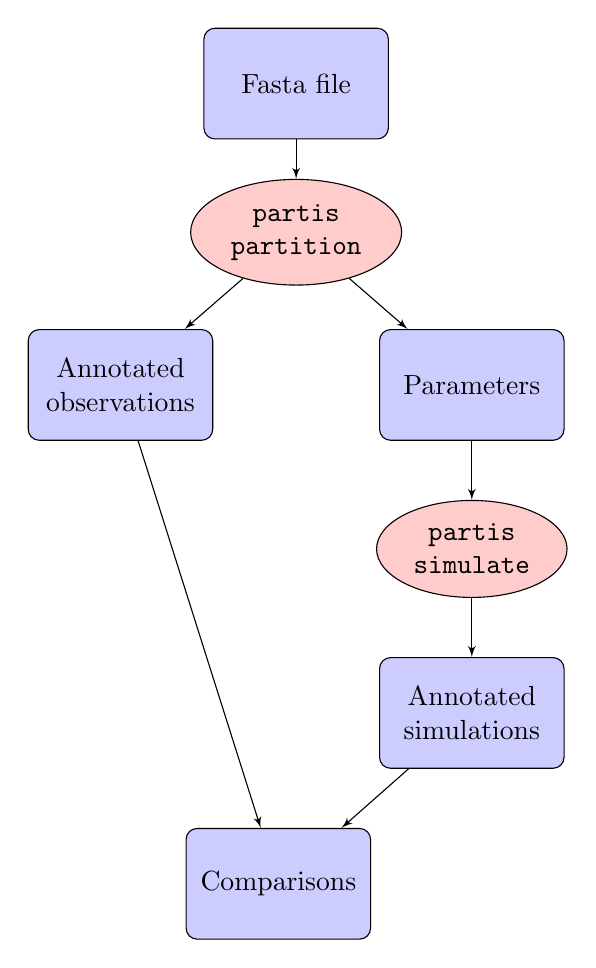
\begin{tikzpicture}
        \node[block](fasta){Fasta file};
        \node[cloud, below =0.5 cm of fasta, align=center](partis){\texttt{partis}\\ \texttt{partition}};
        \node[block, below left=0.75 cm and 0.1 cm of partis](partisdata){Annotated observations};
        \node[block, below right=0.75 cm and 0.1 cm of partis](params){Parameters};
        \node[cloud, below=0.75cm of params, align=center](simulate){\texttt{partis} \\ \texttt{simulate}};
        \node[block, below = 0.75cm of simulate](sim){Annotated simulations};
        \node[block, below left=0.75 and 0.1cm of sim](c1){Comparisons};
        \path[line](fasta) -- (partis);
        \path[line] (partis) -- (partisdata);
        \path[line] (partis) -- (params);
        \path[line] (params) -- (simulate);
        \path[line] (simulate) -- (sim);
        \path[line] (partisdata) -- (c1);
        \path[line] (sim) -- (c1);
    \end{tikzpicture}
\end{adjustbox}
\caption{Workflow for comparing a given observed repertoire dataset to an example simulated dataset via \texttt{partis}.}
\label{PartisWorkflow}
\end{figure}

Next, we discuss a similar model validation approach for TCR repertoires using \texttt{IGoR} \cite{Marcou2018-du}.
We apply IGoR to six datasets from \cite{Britanova2016-iw}, which studied T cell repertoires from donors ranging from newborn children to centenarians.
These datasets consist of consensus RNA sequences assembled using UMIs.
Most of these sequences are functional, and IGoR is meant to build models of nonfunctional sequences that are not biased by selection.
Nonetheless, we believe that meaningful models can be built from this data, and proceed with this caveat in mind.

\subsection*{Scoring summary statistic replication by model}
%EM Would it be worth using some of these figures https://github.com/matsen/talks/tree/gh-pages/figures/sumrep ? (I just invited you.) I think that we're used to this framework but it may be a little strange for others.
%BJO Yes! Though I might have to put this off until after the WG meeting.
We would like a measure of how well a statistic is replicated when a model performs simulations using parameters infered from the observed repertoire dataset.
One approach is to score the statistic $s$ based on the average divergence of observations to their simulated counterparts, and the average divergence of observations to other observations.
Let $\mathcal I$ be the set of dataset indices so that each separate dataset for a (individual, timepoint) pair corresponds to a unique index.
Furthermore, let $R_{i, \text{obs}}$ and $R_{i, \text{sim}}$ be the $i$th observed and simulated repertoire, respectively, and $\mathcal D(R_1, R_2; s)$ be the divergence of repertoires $R_1$ and $R_2$ based on statistic $s$, we have
\begin{equation}
    \text{score}_\text{obs}(s) := \log \left( \frac{ \frac{1}{|\mathcal I|} \sum_{i \in \mathcal I} \mathcal D \left( R_{i, \text{obs}}, R_{i, \text{sim}} ; s\right) }
    { \frac{1}{\frac{1}{2} |\mathcal I|\left(|\mathcal I| - 1\right)}
        \sum_{\substack{i, j \in \mathcal I \\ i \ne j}} \mathcal D\left(R_{i, \text{obs}}, R_{j, \text{obs}}; s\right) } \right)
\end{equation}
This value for a given summary will be negative if \texttt{partis} simulated repertoires tend to look more like their experimental counterparts in terms of this summary than experimental repertoires look like other experimental repertoires, and positive if the experimental repertoires tend to look more alike.

Another related score would be comparing the average divergence of observations to their simulated counterparts, and the average divergence of simulations to other simulations.
Formally, this is
\begin{equation}
    \text{score}_\text{sim}(s) := \log \left( \frac{ \frac{1}{|\mathcal I|} \sum_{i \in \mathcal I} \mathcal D \left( R_{i, \text{obs}}, R_{i, \text{sim}} ; s\right) }
    { \frac{1}{\frac{1}{2} |\mathcal I|\left(|\mathcal I| - 1\right)}
        \sum_{\substack{i, j \in \mathcal I \\ i \ne j}} \mathcal D\left(R_{i, \text{sim}}, R_{j, \text{sim}}; s\right) } \right)
\end{equation}
This value for a given summary will be negative if \texttt{partis} simulated repertoires tend to look more like their experimental counterparts in terms of this summary than simulated repertoires look like other simulated repertoires, and positive if the simulated repertoires tend to look more alike.

\subsection*{Materials}
Table \ref{tab:Datasets} gives metadata for each dataset used in the following analyses.
The raw data were obtained from \cite{Laserson2014-dx}, and the processed data, courtesy of Jason, are from a paper that isn't out yet.
These datasets represent repertoires of patients at various time points following an influenza vaccination.
\begin{table}
\makebox[\textwidth][c]{
\begin{tabular}{c|c|c|c|c|c}
	Dataset label & Dataset type & Annotation tool & Germline set & Individual & Time point \\
	\hline
    \texttt{p\_f1} & Observation &     \texttt{partis} & \texttt{partis} & F & 1 hour \\
    \texttt{p\_f2} & Observation &     \texttt{partis} & \texttt{partis} & F & 8 days \\
    \texttt{p\_g1} & Observation &     \texttt{partis} & \texttt{partis} & G & 1 hour \\
    \texttt{p\_g2} & Observation &     \texttt{partis} & \texttt{partis} & G & 8 days \\
    \texttt{p\_i1} & Observation &     \texttt{partis} & \texttt{partis} & I & 1 hour \\
    \texttt{p\_i2} & Observation &     \texttt{partis} & \texttt{partis} & I & 8 days \\
    \texttt{i\_f1} & Observation &     \texttt{igblast} & \texttt{igblast} & F & 1 hour \\
    \texttt{i\_f2} & Observation &     \texttt{igblast} & \texttt{igblast} & F & 8 days \\
    \texttt{i\_g1} & Observation &     \texttt{igblast} & \texttt{igblast} & G & 1 hour\\
    \texttt{i\_g2} & Observation &     \texttt{igblast} & \texttt{igblast} & G & 8 days\\
    \texttt{i\_i1} & Observation &     \texttt{igblast} & \texttt{igblast} & I & 1 hour\\
    \texttt{i\_i2} & Observation &     \texttt{igblast} & \texttt{igblast} & I & 8 days\\
    \texttt{pi\_f1} & Observation &    \texttt{partis} & \texttt{igblast} & F & 1 hour\\
    \texttt{pi\_f2} & Observation &    \texttt{partis} & \texttt{igblast} & F & 8 days\\
    \texttt{pi\_g1} & Observation &    \texttt{partis} & \texttt{igblast} & G & 1 hour\\
    \texttt{pi\_g2} & Observation &    \texttt{partis} & \texttt{igblast} & G & 8 days\\
    \texttt{pi\_i1} & Observation &    \texttt{partis} & \texttt{igblast} & I & 1 hour\\
    \texttt{pi\_i2} & Observation &    \texttt{partis} & \texttt{igblast} & I & 8 days\\
    \texttt{p\_f1\_sim} & Simulation & \texttt{partis} & \texttt{partis} & F & 1 hour\\
    \texttt{p\_f2\_sim} & Simulation & \texttt{partis} & \texttt{partis} & F & 8 days\\
    \texttt{p\_g1\_sim} & Simulation & \texttt{partis} & \texttt{partis} & G & 1 hour\\
    \texttt{p\_g2\_sim} & Simulation & \texttt{partis} & \texttt{partis} & G & 8 days\\
    \texttt{p\_i1\_sim} & Simulation & \texttt{partis} & \texttt{partis} & I & 1 hour\\
    \texttt{p\_i2\_sim} & Simulation & \texttt{partis} & \texttt{partis} & I & 8 days\\
    \texttt{pi\_f1\_sim} & Simulation& \texttt{partis} & \texttt{igblast} & F & 1 hour\\
    \texttt{pi\_f2\_sim} & Simulation& \texttt{partis} & \texttt{igblast} & F & 8 days\\
    \texttt{pi\_g1\_sim} & Simulation& \texttt{partis} & \texttt{igblast} & G & 1 hour\\
    \texttt{pi\_g2\_sim} & Simulation& \texttt{partis} & \texttt{igblast} & G & 8 days\\
    \texttt{pi\_i1\_sim} & Simulation& \texttt{partis} & \texttt{igblast} & I & 1 hour\\
    \texttt{pi\_i2\_sim} & Simulation& \texttt{partis} & \texttt{igblast} & I & 8 days\\
\end{tabular}
}
\caption{Metadata for each dataset used in the analyses.}
\label{tab:Datasets}
\end{table}
In short, the notation is as follows.
A prefix of \texttt{p} corresponds to \texttt{partis} annotations, a prefix of \texttt{i} corresponds to \texttt{igblast} annotations, and a prefix of \texttt{pi} corresponds to \texttt{partis} annotations using the default \texttt{igblast} germline databases;
this is followed by a letter representing the individual succeeded by a number corresponding to the time point;
finally, we append the \texttt{sim} suffix if the dataset was simulated from an individual's inferred model parameters.

\section*{Results}

\subsection*{Implementation}
The full \texttt{sumrep} package along with the following analyses can be found at \texttt{https://github.com/matsengrp/sumrep}.
It supports BCR and TCR repertoire datasets.
It is open-source, unit-tested, fully documented, and AIRR compliant (by the time of release).
Analyses will be reproducible using Docker.

\texttt{sumrep} contains a function to retrieve each summary statistic in Table \ref{tab:SummaryStatistics}.
A general-purpose implementation of algorithm \ref{DistributionAveraging} is also available and incorporated in applicable summary distributions.
Algorithm \ref{NNDistributionAveraging} is also included for the nearest neighbor distance distribution, which uses \texttt{vsearch} for the clustering routine \cite{Rognes2016-bl}.

\texttt{sumrep} also contains a plotting function for each univariate summary distribution, as well as a master plotting function, \texttt{plotUnivariateDistributions}, which shows a gridded figure of univariate distribution plots.
Currently, these plots can be frequency polygons or empirical cumulative distribution functions.
Each available univariate distribution is plotted by default, although the user can easily specify a custom subset of these distributions.
Figure \ref{fig:MasterPlot} shows an example outputs of \texttt{plotUnivariateDistributions} computed for four datasets: \texttt{p\_f1}, \texttt{p\_f1\_sim}, \texttt{p\_g1}, and \texttt{p\_g1\_sim}.
This function displays frequency polygons by default, but can also display empirical cumulative distribution functions, shown in \ref{fig:MasterPlotECDF} for the same four datasets.
\begin{figure}
    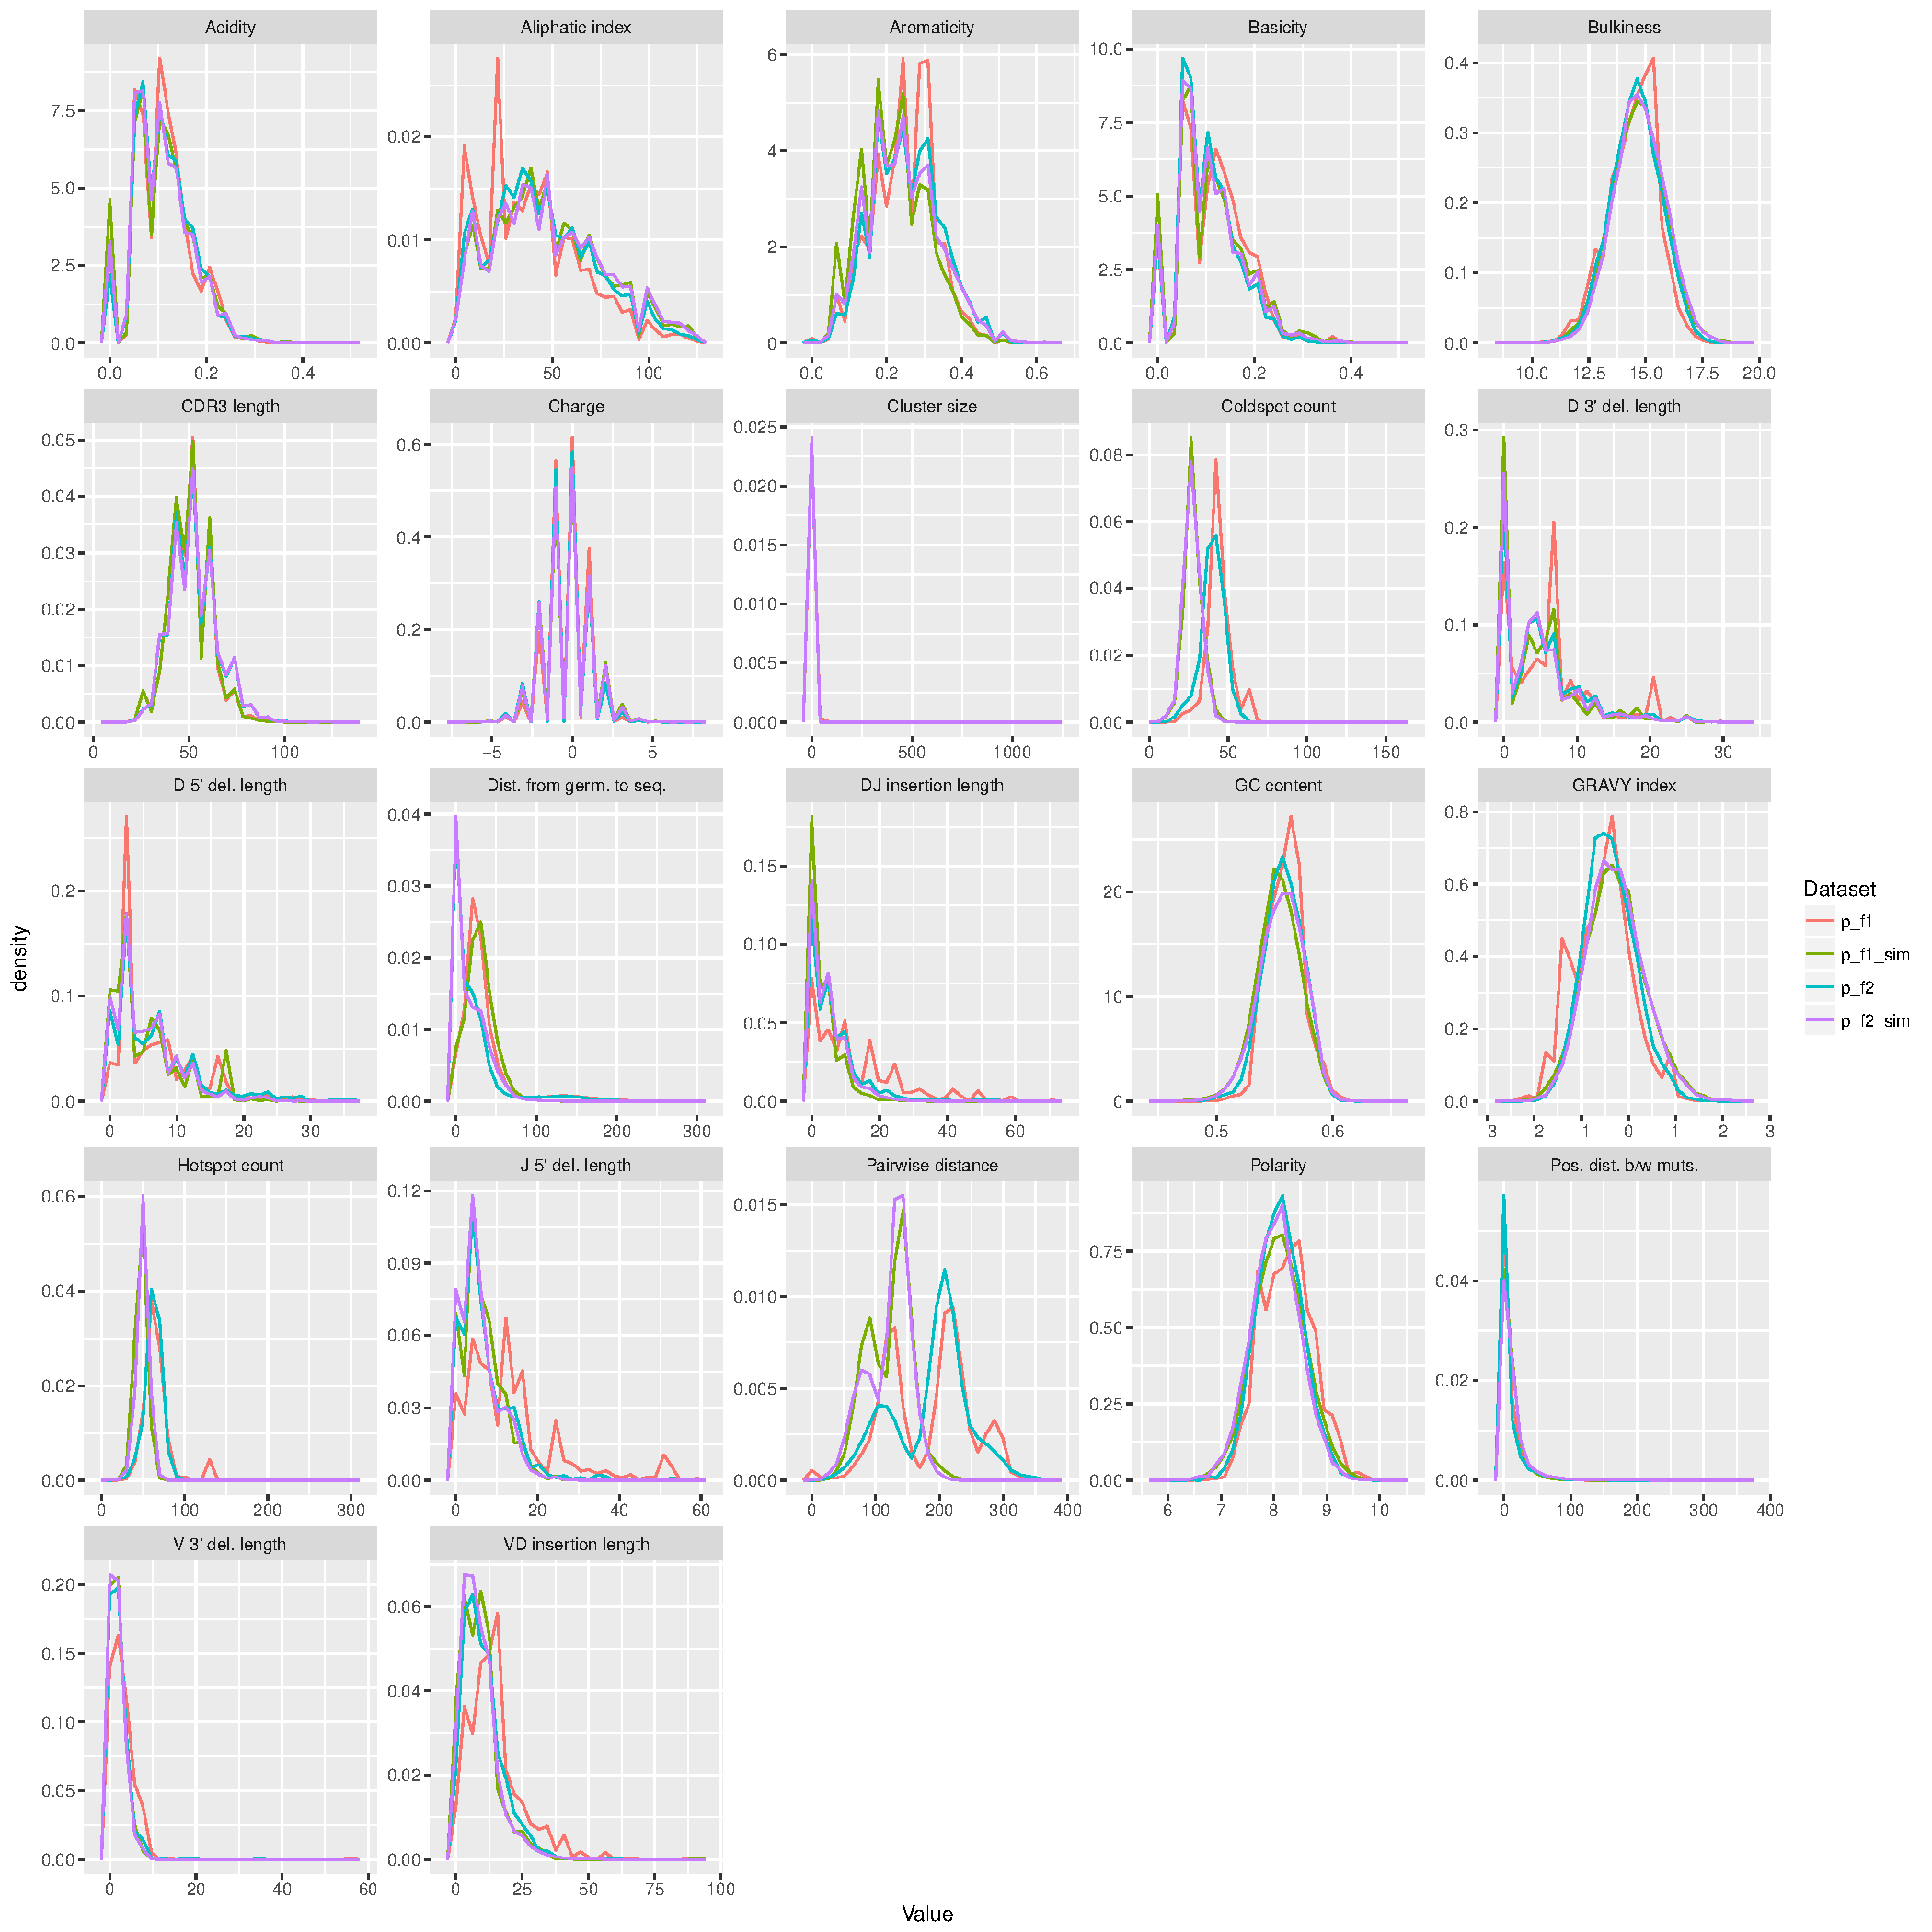
\includegraphics[width=\linewidth]{Figures/master_plot_freqpoly.pdf}
    \caption{Frequency polygon plots of each univariate summary distribution for the \texttt{p\_f1}, \texttt{p\_f1\_sim}, \texttt{p\_g1}, and \texttt{p\_g1\_sim} datasets.}
    \label{fig:MasterPlot}
\end{figure}

\begin{figure}
    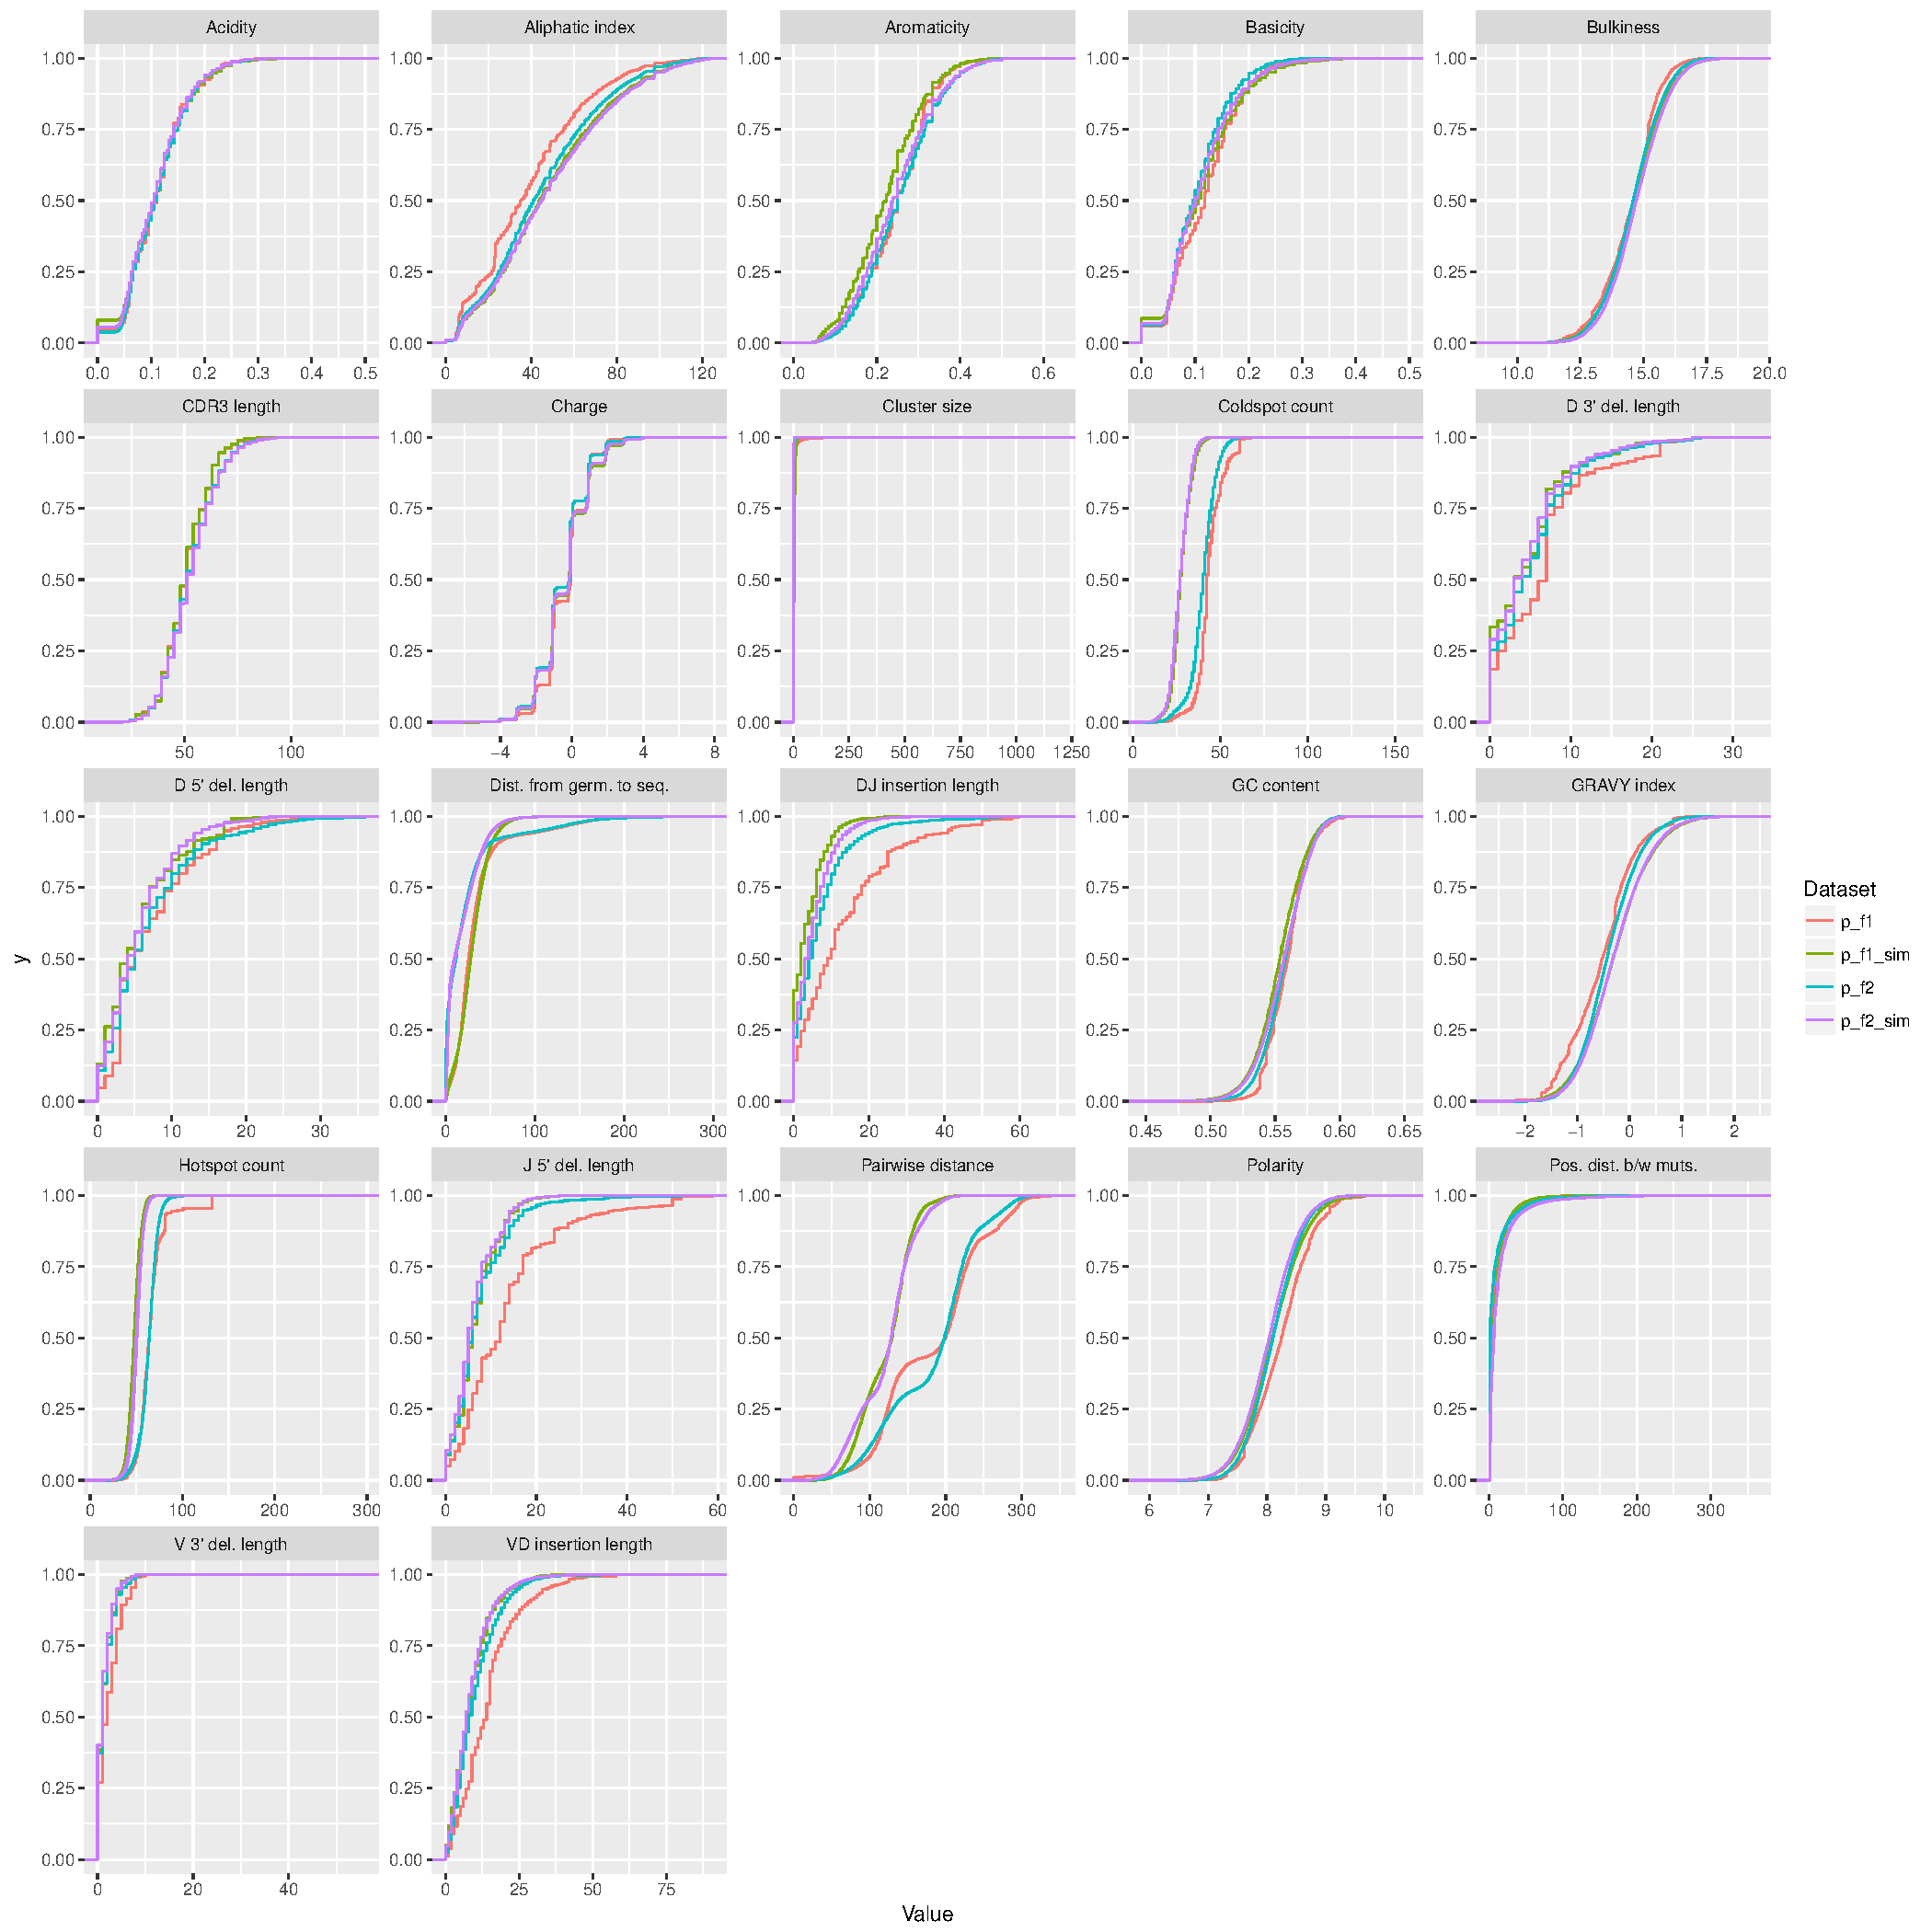
\includegraphics[width=\linewidth]{Figures/master_plot_ecdf.pdf}
    \caption{Empirical cumulative distribution function plots of each univariate summary distribution for the \texttt{p\_f1}, \texttt{p\_f1\_sim}, \texttt{p\_g1}, and \texttt{p\_g1\_sim} datasets.}
    \label{fig:MasterPlotECDF}
\end{figure}

\subsection*{Model validation}

%EM Results paragraphs concern what was found. Can you comment on overall trends or interesting things we found that people can find in the figure?
Figure \ref{fig:SimObs} displays the divergences of each statistic in \ref{tab:SummaryStatistics} for three observed repertoires.
\begin{figure}
    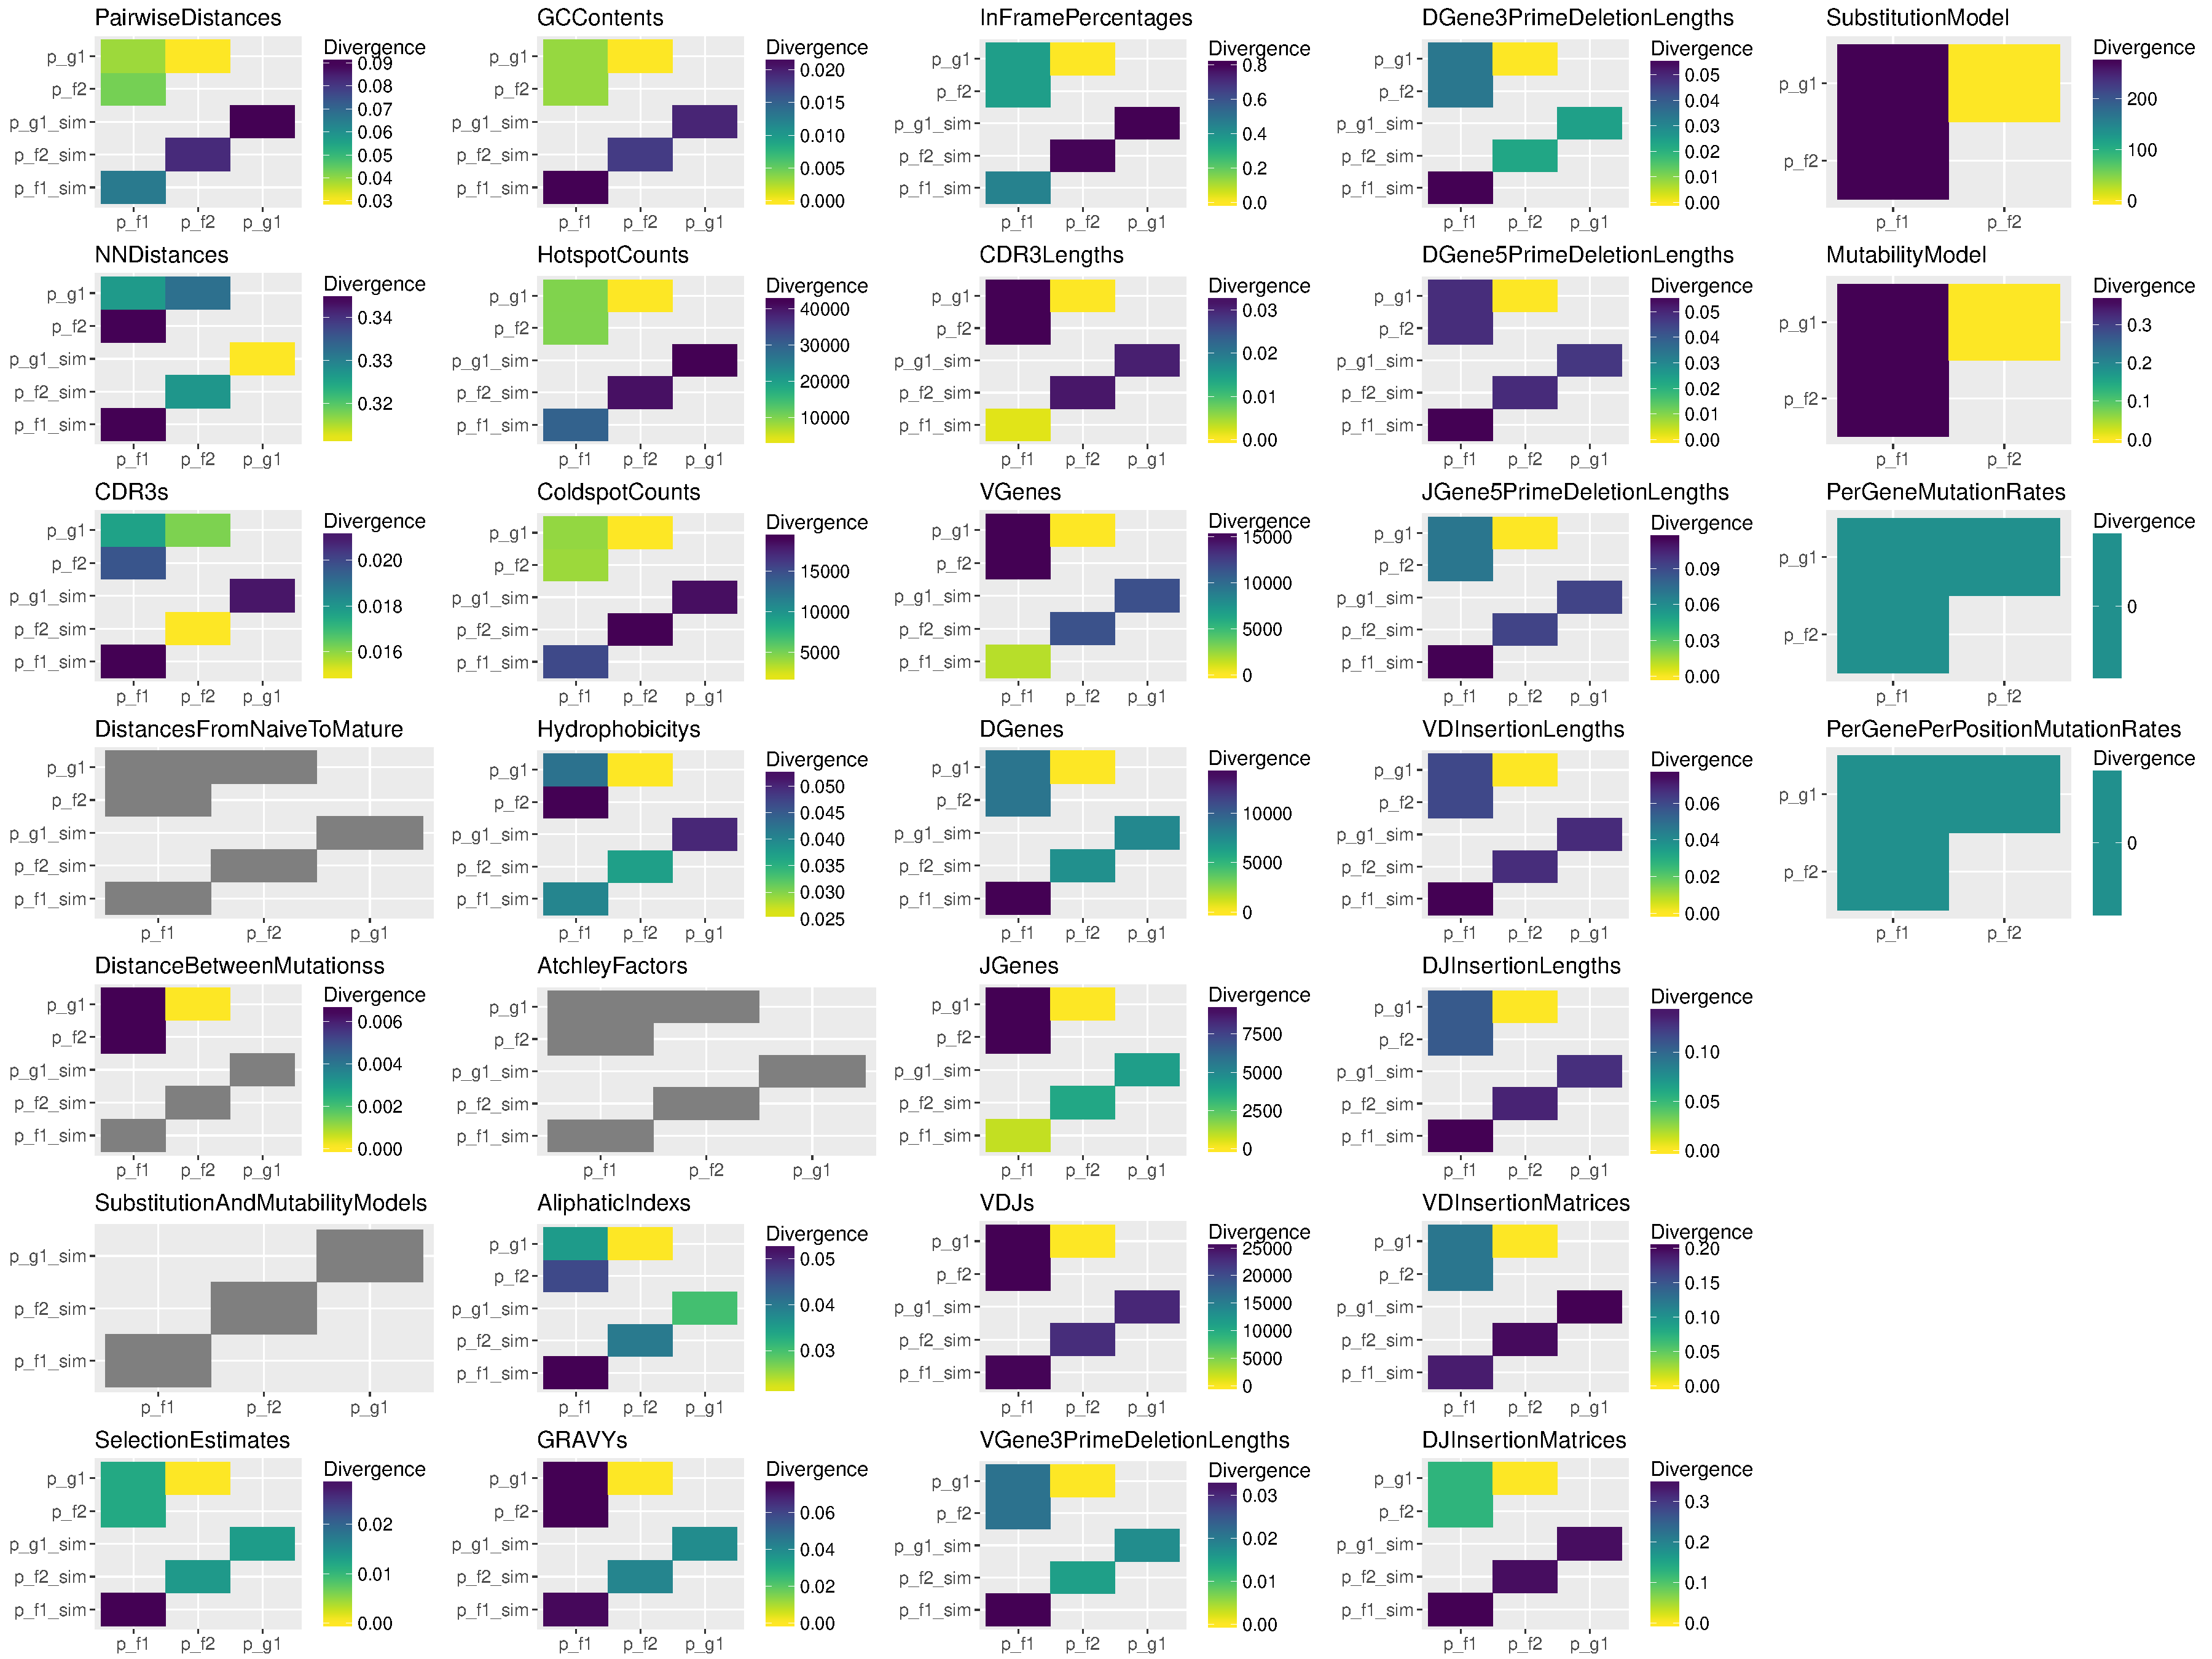
\includegraphics[width=\linewidth]{Figures/sim_obs.pdf}
    \caption{Divergences of empirical summary distributions based on three individual observed datasets.}
    \label{fig:SimObs}
\end{figure}
Because the absolute divergence values are sensitive to scale as well as the type of divergence used, we also include divergences for each observation-observation pair as a benchmark.
The idea here is that a very good simulator should result in low divergence values between its reference repertoire and its simulated repertoire, as opposed to comparing the observed dataset to any other dataset.
For such a simulator, the diagonal at the bottom of the plots in figure \ref{fig:SimObs}, which represents observation-simulation divergences, would have lighter colors than those in the upper left corner, which represent observation-observation divergenes.
We see that this is the case for some statistics, particularly the germline gene usages and CDR3 lengths, but in other cases the observations tend to be more similar to other observations, such as for the distributions of positional distance between mutations.

A valid concern about our methodology is that \texttt{partis} simulations would be unreasonably biased by \texttt{partis} annotations on which they are based.
To address this, we performed dataset annotation using standalone \texttt{igblast} \cite{Ye2013-kl}, and compared these to simulations based on \texttt{partis} annotations using the \texttt{igblast} germline databases.
Change-O was used to parse the \texttt{igblast} output \cite{Gupta2015-iu}.
Our strategy is analogous to the one above but with the inclusion of a separate path for \texttt{igblast} annotations.
The workflow for this procedure is displayed in figure \ref{IgblastWorkflow}.
\begin{figure}
    \begin{adjustbox}{max totalsize={\textwidth}{.8\textheight},center}
        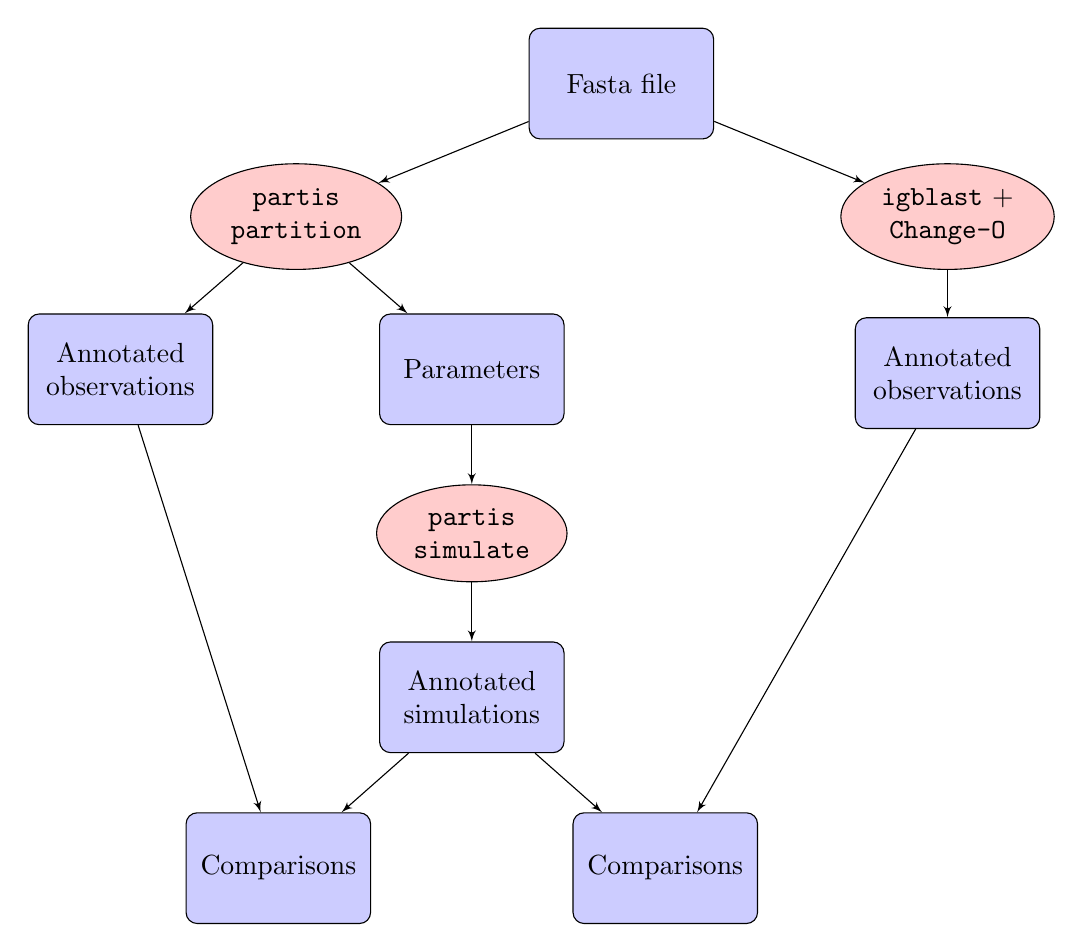
\begin{tikzpicture}
            \node[block](fasta){Fasta file};
            \node[cloud, below left=0.5 cm and 2 cm of fasta, align=center](partis){\texttt{partis}\\ \texttt{partition}};
            \node[cloud, below right=0.5 cm and 2 cm of fasta, align=center](igblast){\texttt{igblast} + \\ \texttt{Change-O}};
            \node[block, below left=0.75 cm and 0.1 cm of partis](partisdata){Annotated observations};
            \node[block, below right=0.75 cm and 0.1 cm of partis](params){Parameters};
            \node[cloud, below=0.75cm of params, align=center](simulate){\texttt{partis} \\ \texttt{simulate}};
            \node[block, below = 0.75cm of simulate](sim){Annotated simulations};
            \node[block, below=0.6 cm of igblast](igblastdata){Annotated observations};
            \node[block, below left=0.75 and 0.1cm of sim](c1){Comparisons};
            \node[block, below right=0.75 and 0.1cm of sim](c2){Comparisons};
            \path[line](fasta) -- (partis);
            \path[line](fasta) -- (igblast);
            \path[line] (partis) -- (partisdata);
            \path[line] (partis) -- (params);
            \path[line] (igblast) -- (igblastdata);
            \path[line] (params) -- (simulate);
            \path[line] (simulate) -- (sim);
            \path[line] (partisdata) -- (c1);
            \path[line] (sim) -- (c1);
            \path[line] (igblastdata) -- (c2);
            \path[line] (sim) -- (c2);
        \end{tikzpicture}
    \end{adjustbox}
    \caption{Workflow for comparing \texttt{partis} and \texttt{igblast} annotations to partis simulations}
    \label{IgblastWorkflow}
\end{figure}
The results are displayed in figure \ref{PartisIgb}.
\begin{figure}
    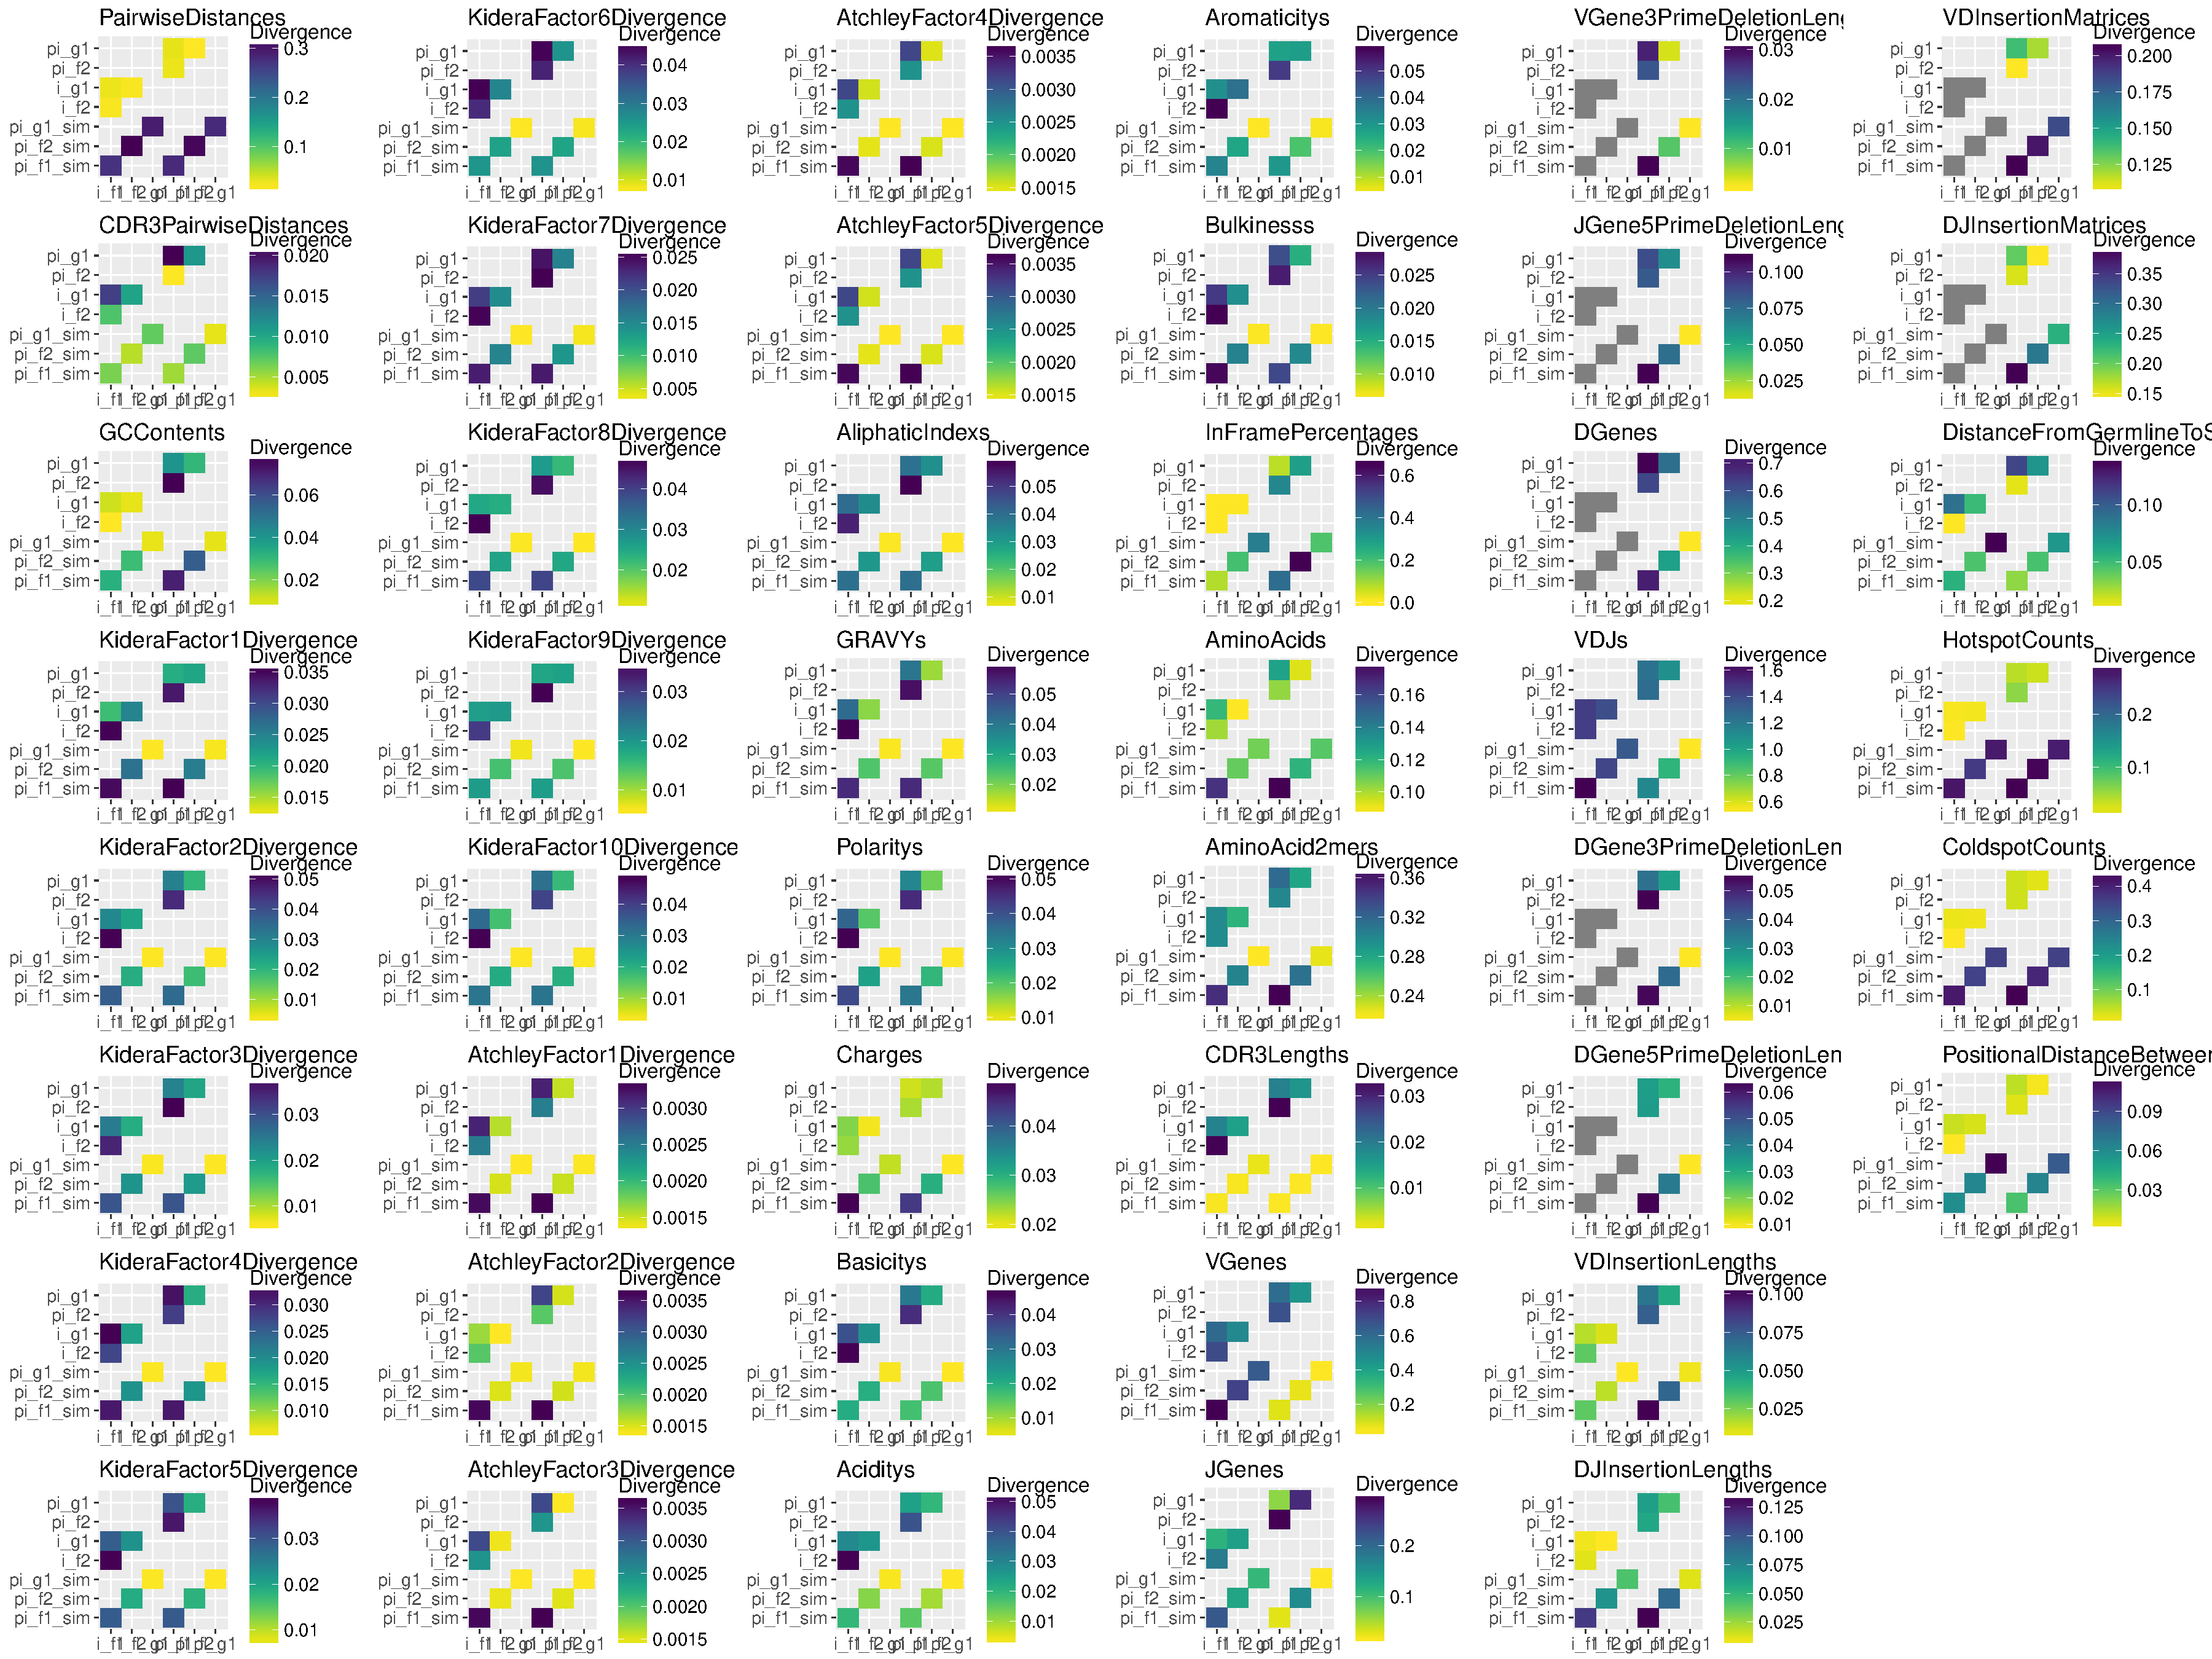
\includegraphics[width=\linewidth]{Figures/partis_igb.pdf}
    \caption{Comparing divergences for \texttt{igblast} annotations and \texttt{partis} simulations based on the same individual observed repertoires.
        We use the default germline databases in \texttt{igblast} for consistency.
    }
    \label{PartisIgb}
\end{figure}
The plots do not suggest any systematic bias in our approach.


\subsection*{Assessing summary statistic replication for \texttt{partis}}
%EM Need some text here describing what was found.
Figure \ref{fig:ObsScoresBCR} displays the observation-based summary scores for the six BCR datasets based on \texttt{partis} simulations.
\begin{figure}
    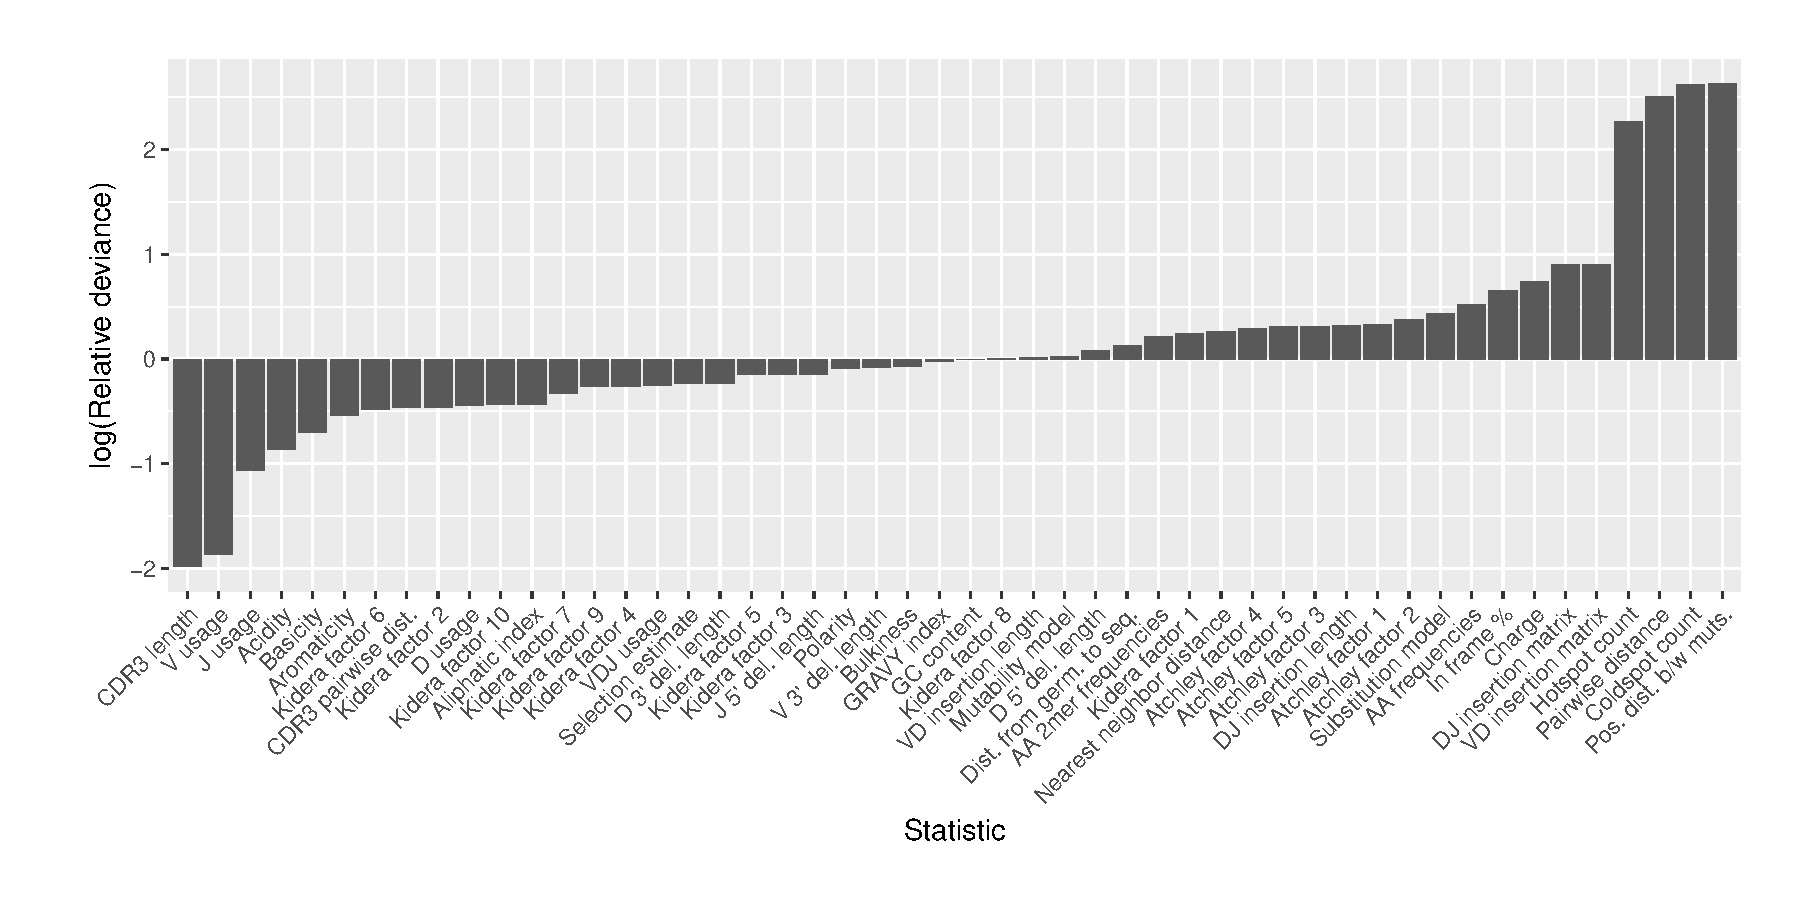
\includegraphics[width=\linewidth]{Figures/obs_score_plot.pdf}
    \caption{$\text{score}_\text{obs}$ of each statistic based on \texttt{partis} model inference and simulation.
        A low score indicates a well-replicated statistic by the simulations.
    }
    \label{fig:ObsScoresBCR}
\end{figure}
As noted from Figure \ref{fig:SimObs}, the best-recapitulated statistics tend to be CDR3 lengths and most of the statistics based on germline inferences.
This is sensible as these per-sample statistics are directly used for simulation.
Interestingly, the simulations do tend to capture selection estimates and GRAVY indices well despite these quantities not being involved in the inference or simulation process.
Conversely, the simulations tend to have less agreement in distributions of hotspot and coldspot motifs as well as positional distance between mutations and VD/DJ insertion matrices.

Figure \ref{fig:SimScoresBCR} displays the simulation-based summary scores for the same datasets and simulations.
\begin{figure}
    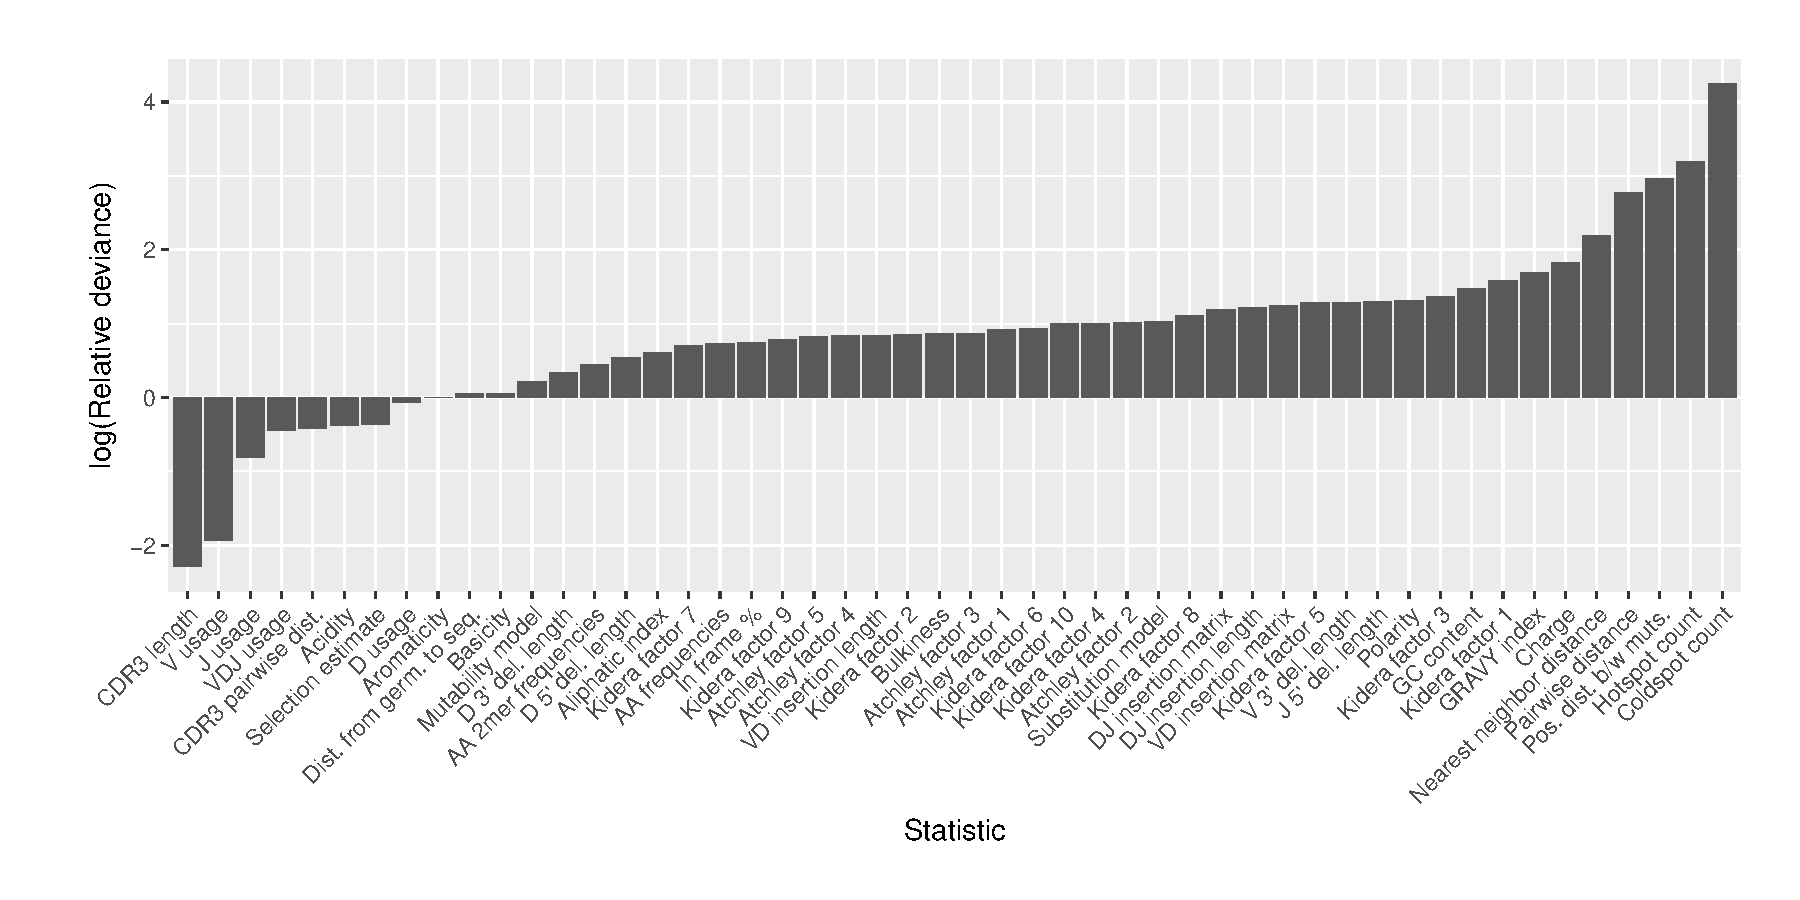
\includegraphics[width=\linewidth]{Figures/sim_score_plot.pdf}
    \caption{$\text{score}_\text{sim}$ of each statistic based on \texttt{partis} model inference and simulation.
        A low score indicates a well-replicated statistic by the simulations.
    }
    \label{fig:SimScoresBCR}
\end{figure}

We see that for the vast majority of summaries, this score is greater than zero, indicating that simulations look closer to other simulations than they do to their experimental counterparts.
While this is not very surprising since model simulations are a simplifiication of the true data-generating process, this does suggest that important biological quantities may need to be explicitly accounted for in a more accurate generative model.

\subsection*{Assessing summary statistic replication for \texttt{igor}}
Figure \ref{fig:ObsScoresTCR} displays the observation-based summary scores for the six TCR datasets based on \texttt{igor} simulations.

\begin{figure}
    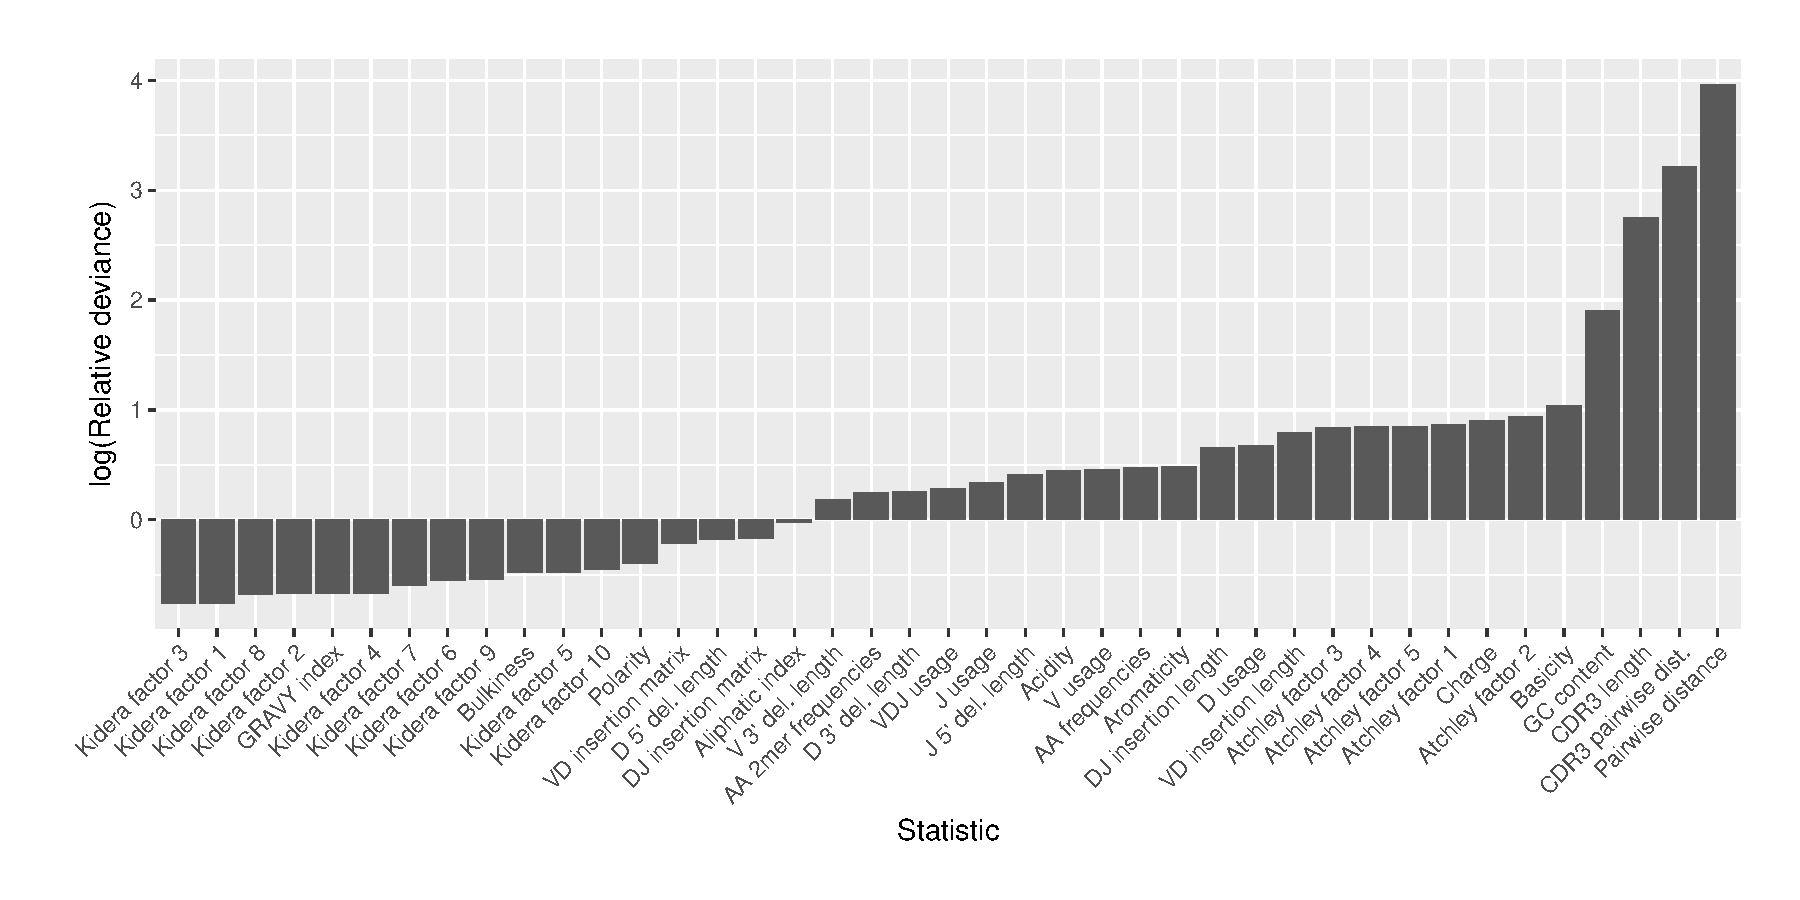
\includegraphics[width=\linewidth]{Figures/obs_score_plot-tcr.pdf}
    \caption{$\text{score}_\text{obs}$ of each statistic based on \texttt{igor} model inference and simulation.
        A low LRD indicates a well-replicated statistic by the simulations.
    }
    \label{fig:ObsScoresTCR}
\end{figure}

Figure \ref{fig:SimScoresBCR} displays the simulation-based summary scores for the same datasets and simulations.
\begin{figure}
    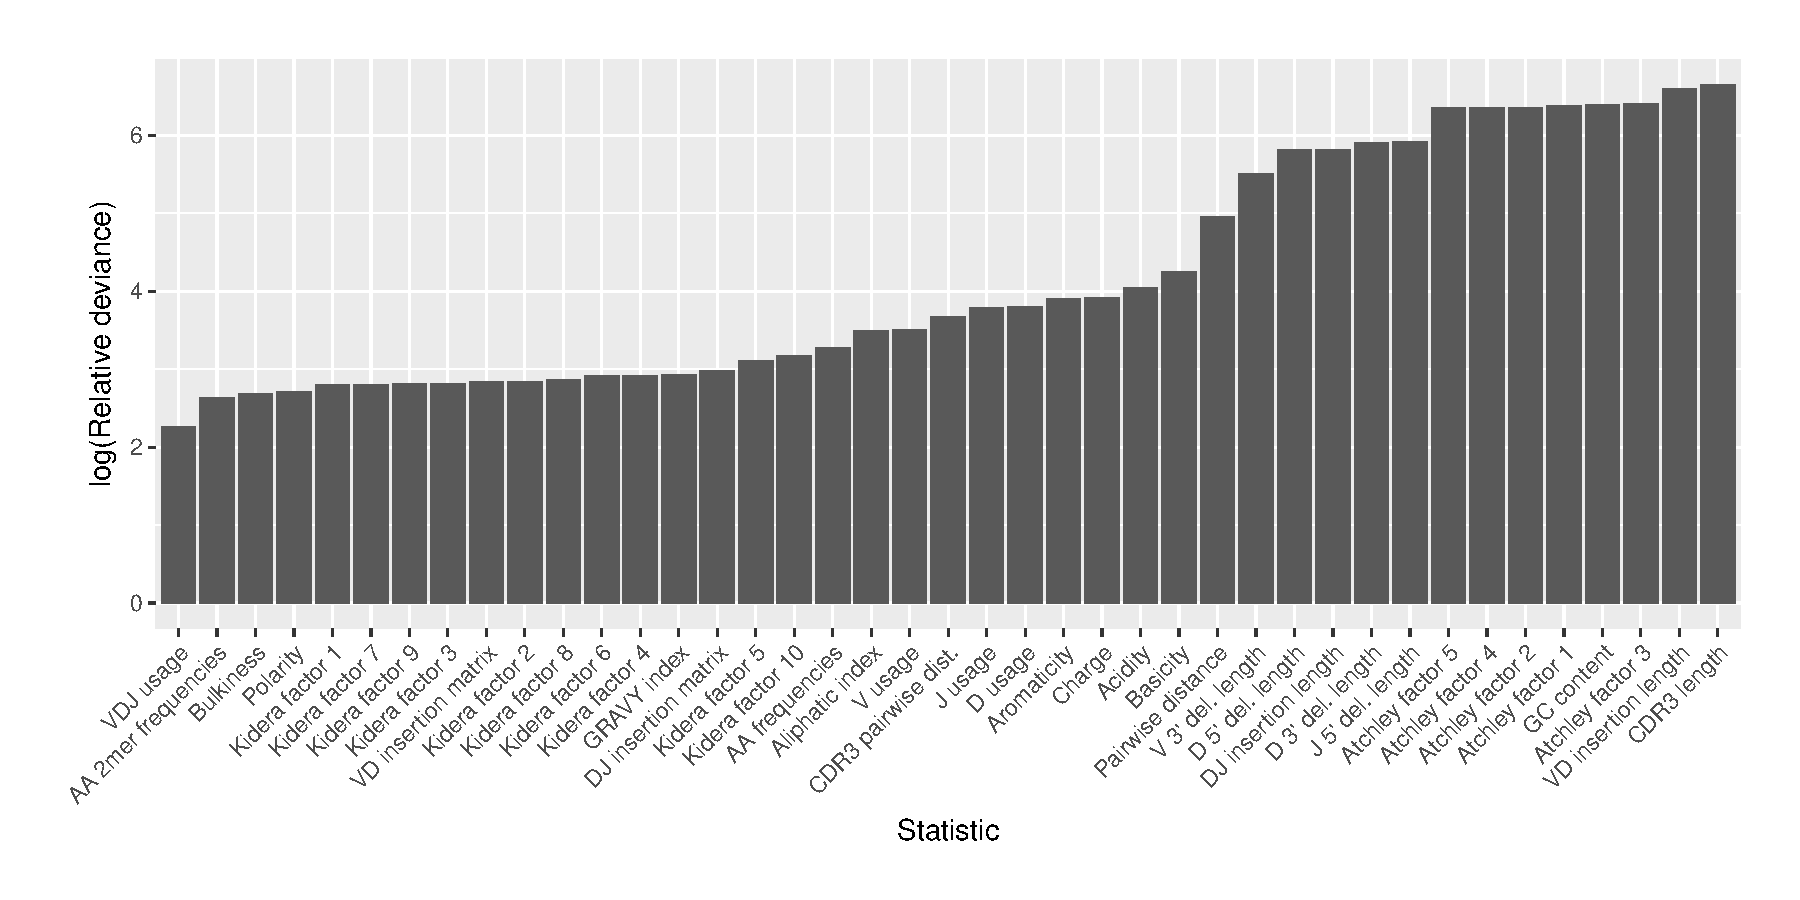
\includegraphics[width=\linewidth]{Figures/sim_score_plot-tcr.pdf}
    \caption{$\text{score}_\text{sim}$ of each statistic based on \texttt{igor} model inference and simulation.
        A low LRD indicates a well-replicated statistic by the simulations.
    }
    \label{fig:SimScoresTCR}
\end{figure}



\subsection*{Comparing observations to competing model simulations}

\section*{Discussion}
We aren't talking about pairwise summary statistics such as UniFrac \cite{De_Bourcy2017-pu}.

\bibliographystyle{plain}
\bibliography{main}

\section*{Appendix A: Performance of distribution subsampling algorithms}
Here, we run Algorithm \ref{DistributionAveraging} on \texttt{p\_f1} subsampled without replacement to 10,000 sequences.
We compute the pairwise distance distribution of CDR3 sequences for the full subsampled dataset, as well as using Algorithm \ref{DistributionAveraging} with tolerances $\varepsilon \in \left\{0.1, 0.001, \dotsc, 10^{-7} \right\}$.
We replicate this experiment for 10 trials so that the subsampled dataset remains the same, but a new instance of the subsampling algorithm is run each time.
Figure \ref{fig:Distributions} displays density estimates of one trial for each of the distributions; visually, it appears that lower tolerances correspond to closer distributions to the true "population" distribution.
\begin{figure}
    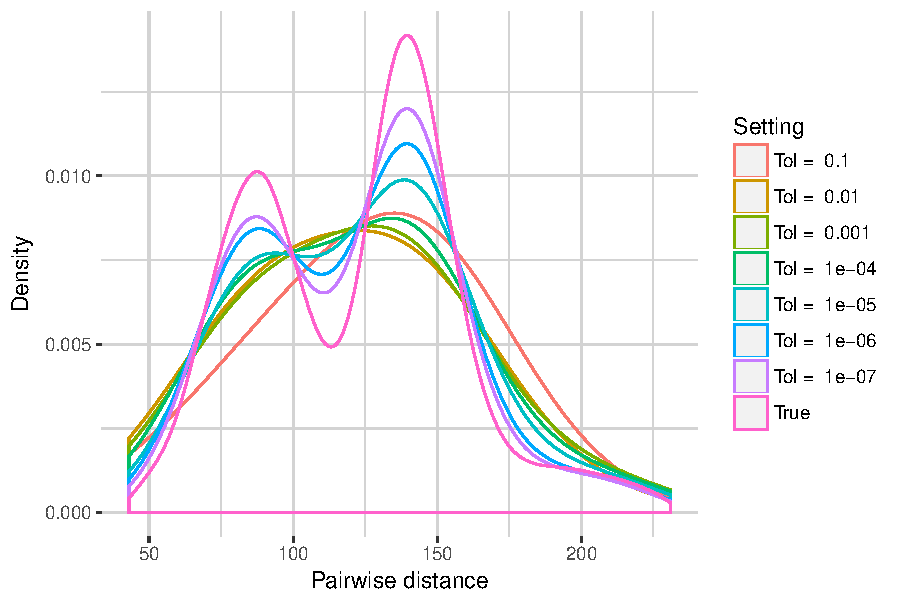
\includegraphics[width=\linewidth]{Figures/PairwiseDistance/density_by_tol.pdf}
    \caption{Density estimates of true and subsampled pairwise distance distributions by tolerance.}
    \label{fig:Distributions}
\end{figure}
However, the density estimates exhibit awkward and inconsistent smoothing based on both the differences in orders of magnitude between distributions, as well as the fact that the pairwise distance distribution takes discrete values (and are thus not well-described by continuous smoothing kernels).
We can instead look at the following more appropriate summaries for discrete data.
Figure \ref{fig:FreqPoly} shows a frequency polygon of the same distributions, and Figure \ref{fig:ECDF} shows their empirical cumulative distribution functions.
\begin{figure}
    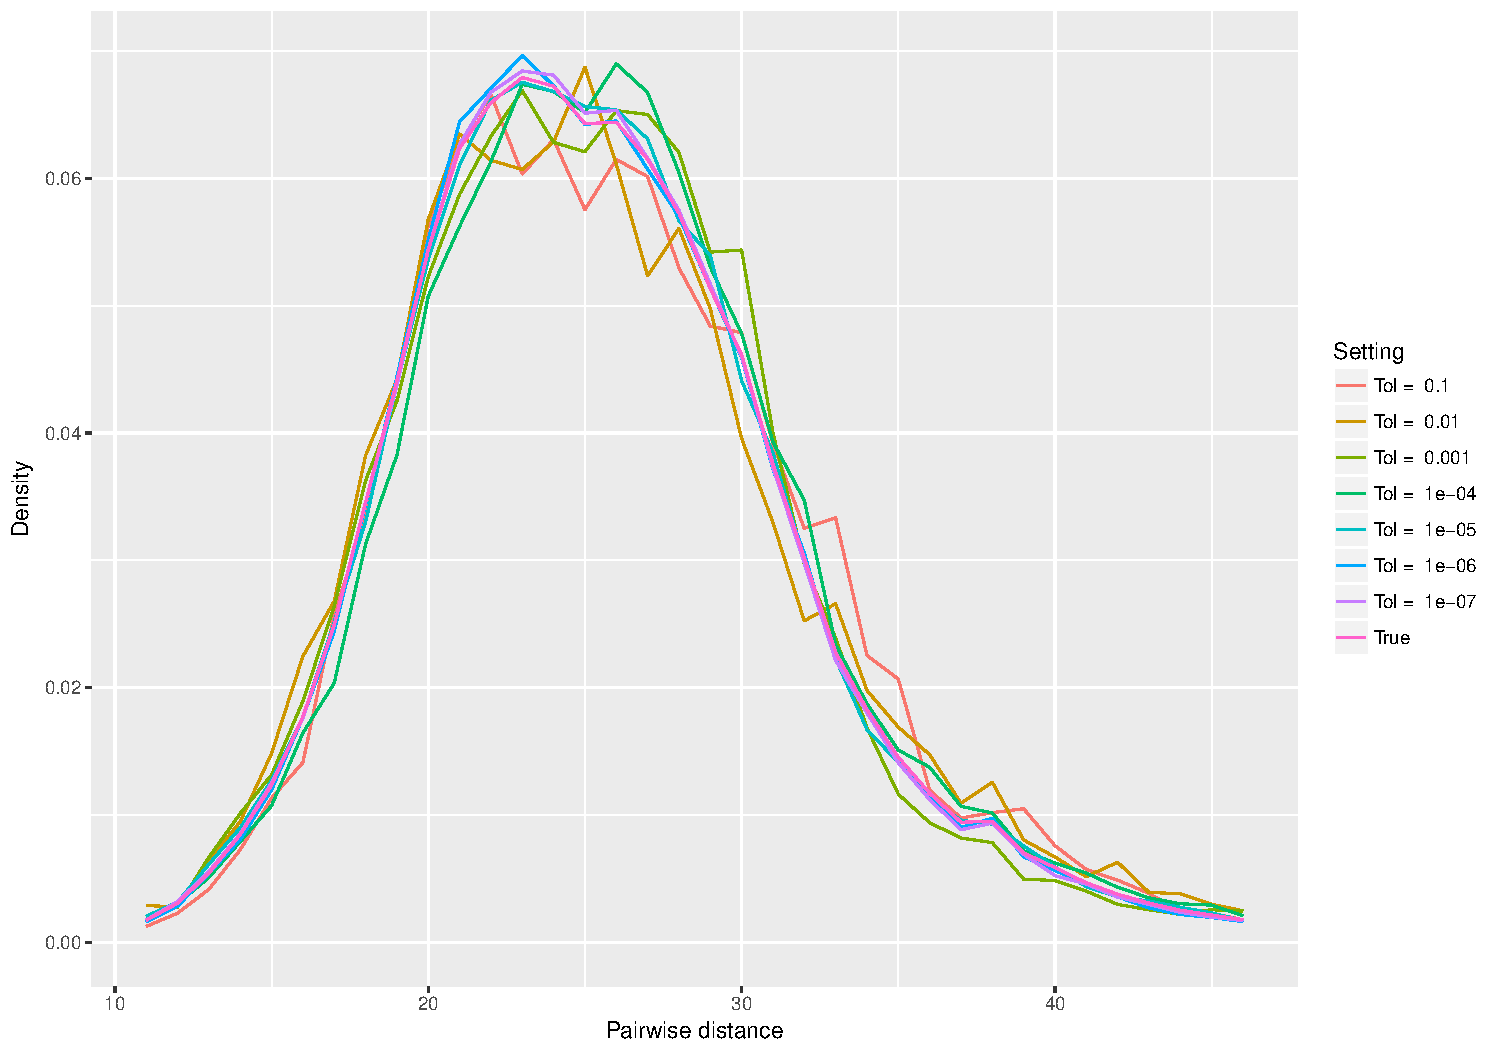
\includegraphics[width=\linewidth]{Figures/PairwiseDistance/freqpoly_by_tol.pdf}
    \caption{Frequency polygons of true and subsampled pairwise distance distributions by tolerance.}
    \label{fig:FreqPoly}
\end{figure}
\begin{figure}
    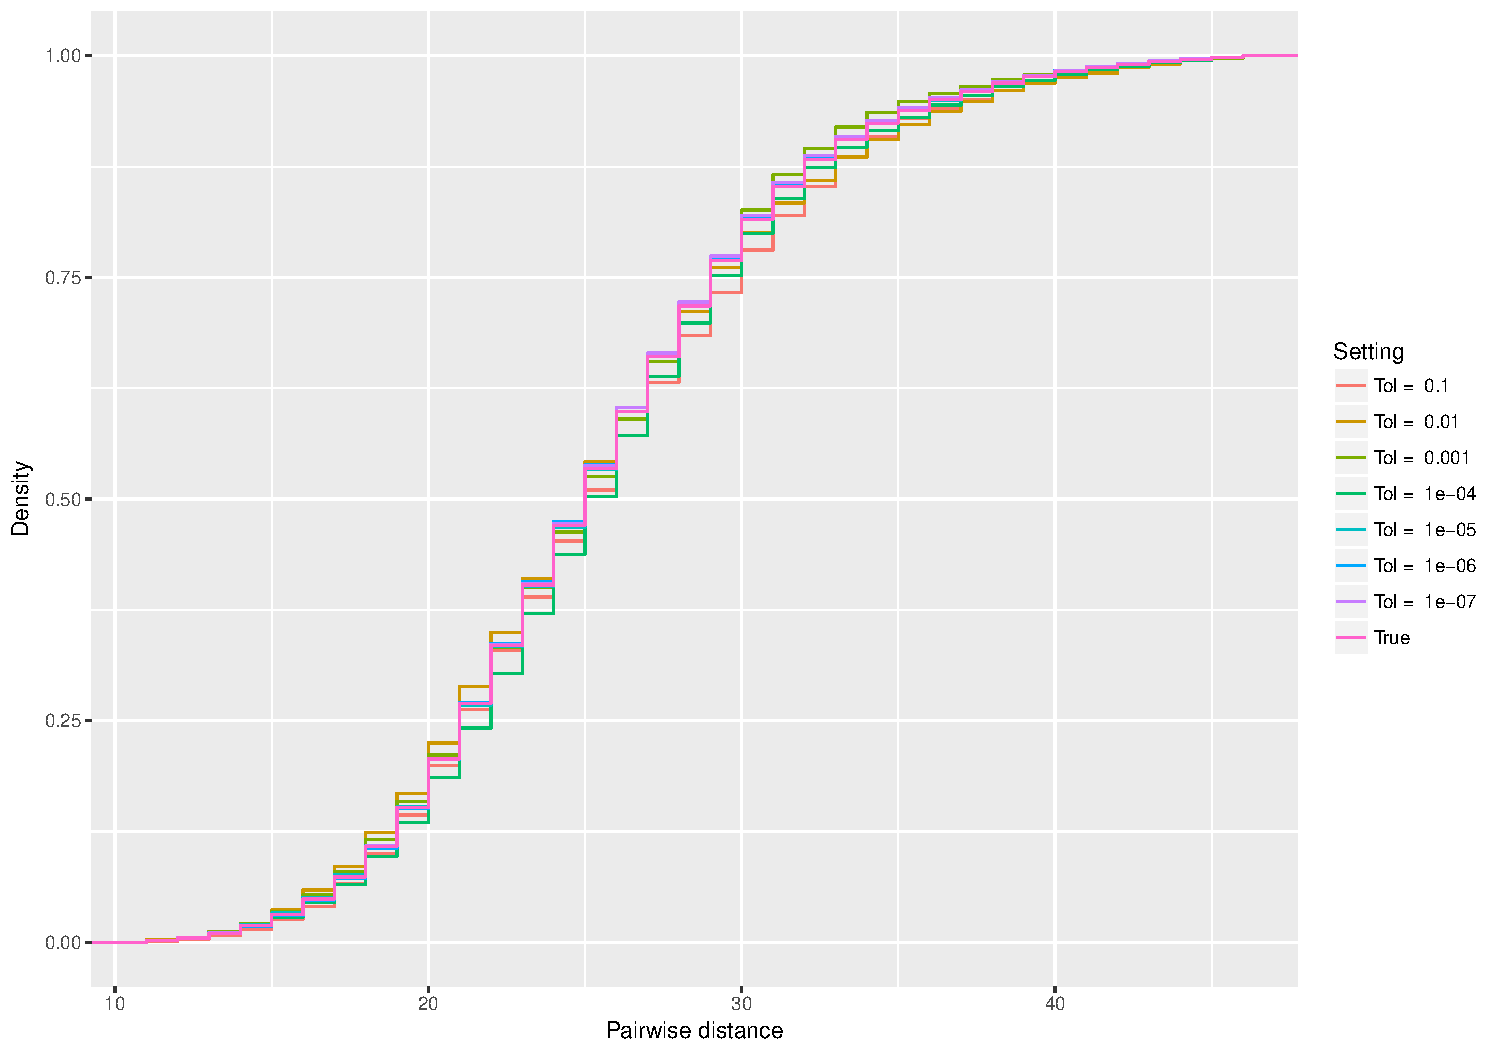
\includegraphics[width=\linewidth]{Figures/PairwiseDistance/ecdf_by_tol.pdf}
    \caption{Empirical c.d.f. of true and subsampled pairwise distance distributions by tolerance.}
    \label{fig:ECDF}
\end{figure}

\begin{center}
% latex table generated in R 3.4.1 by xtable 1.8-2 package
% Thu Oct  4 10:50:34 2018
\begin{tabular}{lrrrrrr}
 Distribution & Min & Q1 & Median & Mean & Q3 & Max \\ 
  \hline
\hline
Tol =  0.1 & 0 & 22 & 25 & 25.55 & 29 & 60 \\ 
  Tol =  0.01 & 0 & 22 & 26 & 26.87 & 30 & 81 \\ 
  Tol =  0.001 & 0 & 21 & 25 & 25.70 & 29 & 73 \\ 
  Tol =  1e-04 & 0 & 21 & 25 & 25.31 & 29 & 64 \\ 
  Tol =  1e-05 & 0 & 21 & 25 & 25.59 & 29 & 78 \\ 
  Tol =  1e-06 & 0 & 21 & 25 & 25.76 & 30 & 108 \\ 
  Tol =  1e-07 & 0 & 21 & 25 & 25.76 & 30 & 84 \\ 
  True & 0 & 21 & 25 & 25.70 & 29 & 116 \\ 
  \end{tabular}
\end{center}
\label{tab:SummaryTable}
Numerical summaries for each distribution are shown in Table \ref{tab:SummaryTable}.

Figure \ref{fig:Divergences} displays the KL-divergence to the true distribution for each tolerance.
\begin{figure}
    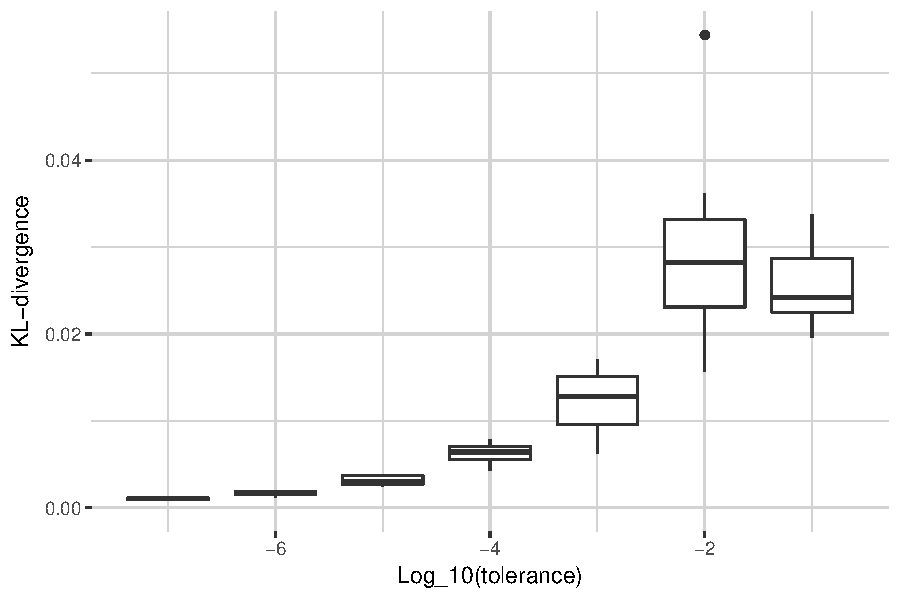
\includegraphics[width=\linewidth]{Figures/PairwiseDistance/div_by_tol.pdf}
    \caption{KL-divergence to true pairwise distance distribution by tolerance, taken over 10 trials of the algorithm.}
    \label{fig:Divergences}
\end{figure}
Figure \ref{fig:Times} displays the runtimes and log-runtimes for each tolerance as well as the true "population" runtime for the full dataset.
\begin{figure}
    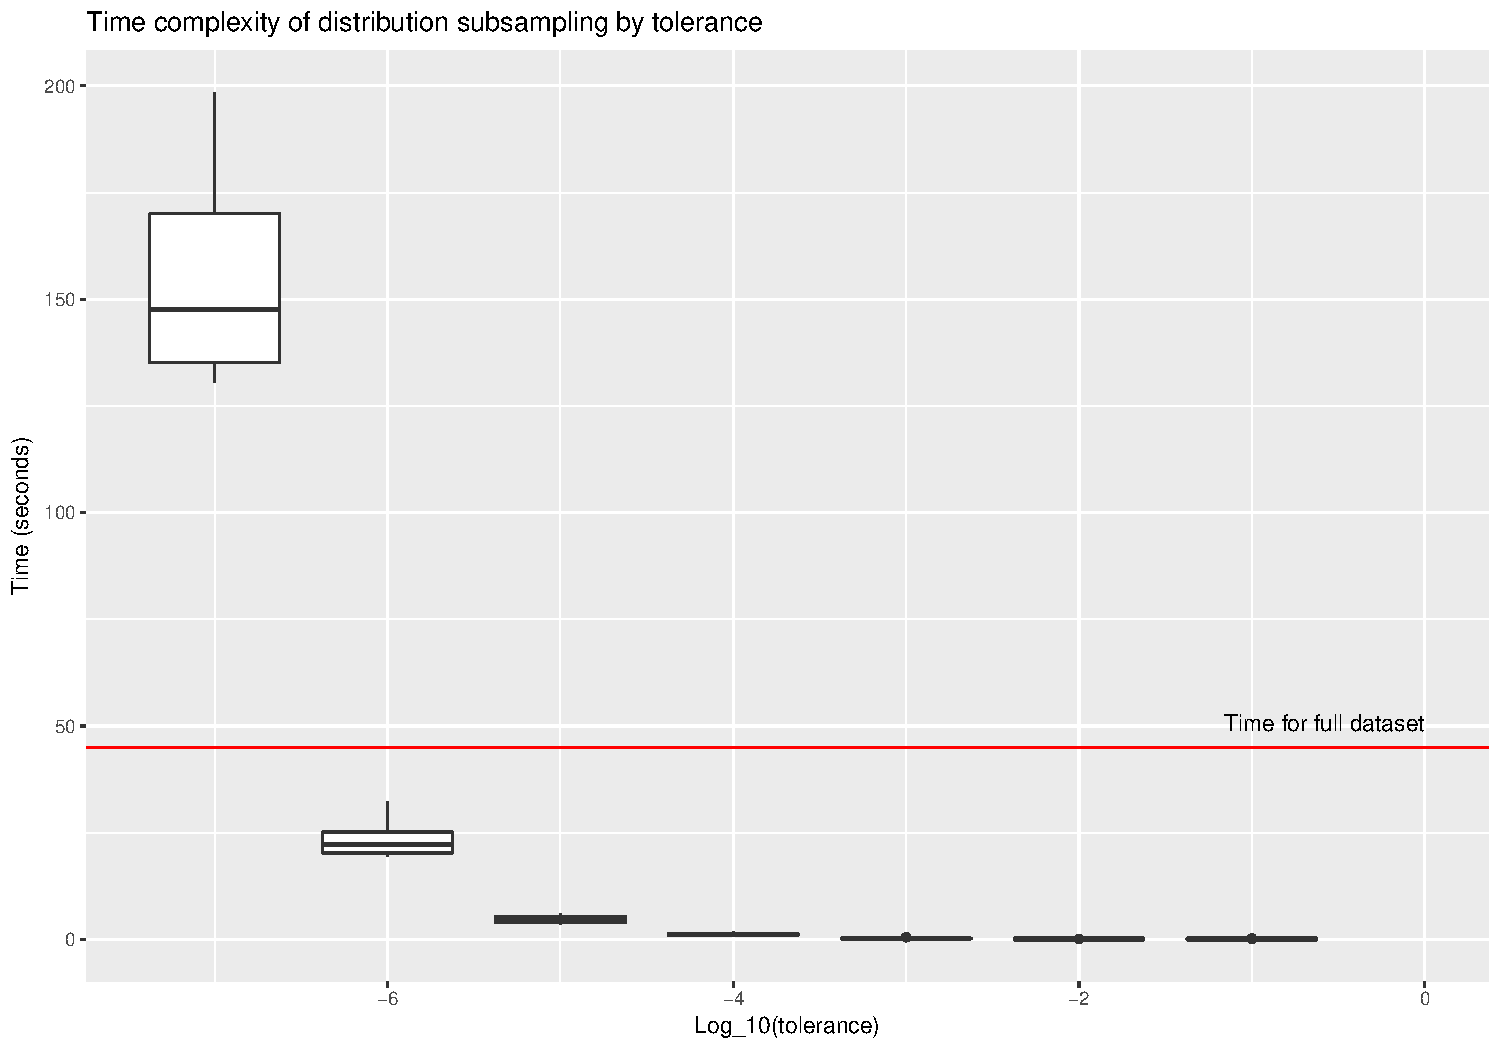
\includegraphics[width=0.9\linewidth]{Figures/PairwiseDistance/time_by_tol.pdf}
    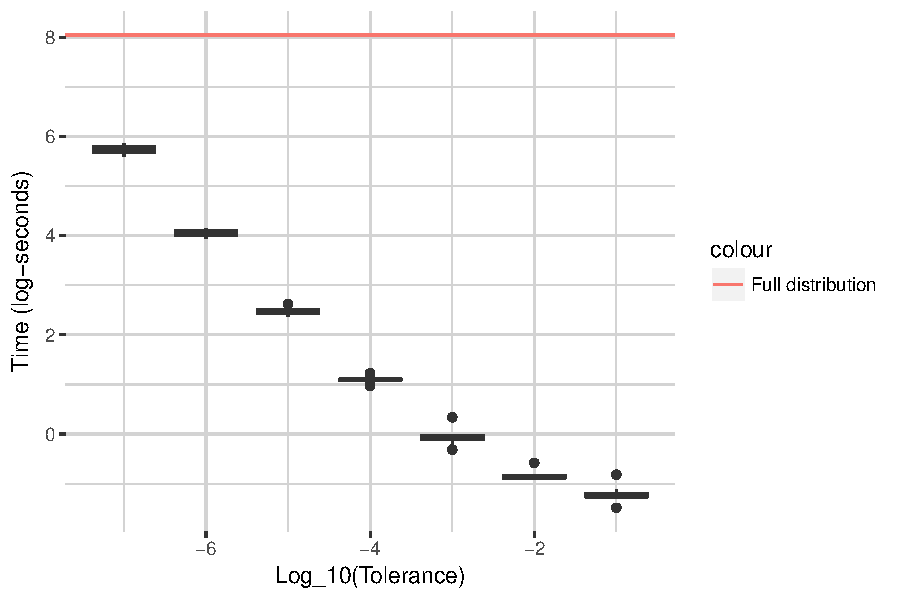
\includegraphics[width=0.9\linewidth]{Figures/PairwiseDistance/log_time_by_tol.pdf}
    \caption{Runtime (in seconds) and log-runtime (in log-seconds) for Algorithm \ref{DistributionAveraging} by tolerance, taken over 10 trials.}
    \label{fig:Times}
\end{figure}


For a tolerance of $\varepsilon = 10^{-3}$, we see that the KL-divergence of the approximate distribution to the true distribution is consistently small, most of the time falling below 0.01. 
Figure \ref{fig:Times} shows that running the algorithm with this tolerance yields an exponentially faster runtime than when computing the full distribution.  
Even the higher tolerances of $\varepsilon = 0.1, 0.01$ yield low KL divergences, although the variability is higher.

Next we investigate the effect of dataset size on the performance of Algorithm \ref{DistributionAveraging}.
For sample sizes $s \in \{\exp(5), \dotsc, \exp(9)\}$, we subsample \texttt{p\_f1} without replacement to $s$ sequences and compute the pairwise distance distribution of CDR3 sequences for the full subsampled dataset as well as those given by tolerances $\varepsilon \in \{0.1, 0.01, 0.001\}$.  
We perform this experiment 10 times for each $s$.
Boxplots of the KL-divergence by log(size) and tolerance over all trials are displayed in Figure \ref{fig:Sizes}.
\begin{figure}
    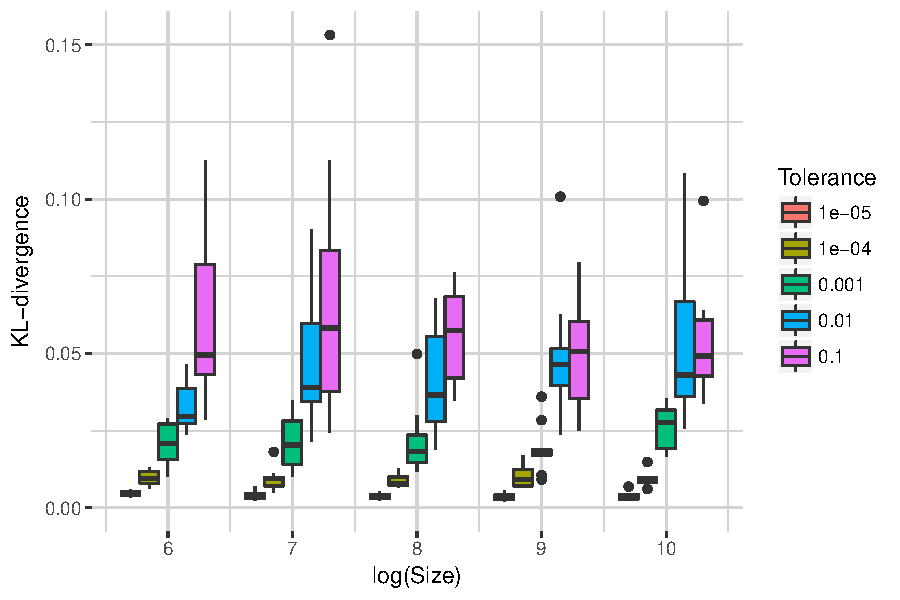
\includegraphics[width=\linewidth]{Figures/PairwiseDistance/div_by_size_and_tol.pdf}
    \caption{KL-divergence to true pairwise distance distribution by tolerance and log(size) of dataset, taken over 10 trials of the algorithm.}
    \label{fig:Sizes}
\end{figure}
The figure shows no obvious trend in the effect of dataset size on the KL-divergence for any choice of tolerance.
This suggests that the accuracy of our procedure is scalable to large datasets.

Finally, we investigate the effect of summary statistic on the performance of Algorithm \ref{DistributionAveraging}.
We run the algorithm for the pairwise distance, GC content, hotspot count, and coldspot count distributions on \texttt{p\_f1} subsampled without replacement to 5,000 rows.
For each summary, we run the algorithm for tolerances $\varepsilon \in \{0.1, \dotsc, 10^{-7}\}$.
We perform this experiment 10 times for each (summary, $\varepsilon$) combination.
Figure \ref{fig:SummaryPerformance} shows the KL-divergence to the full dataset distributions by summary and tolerance over all trials.
\begin{figure}
    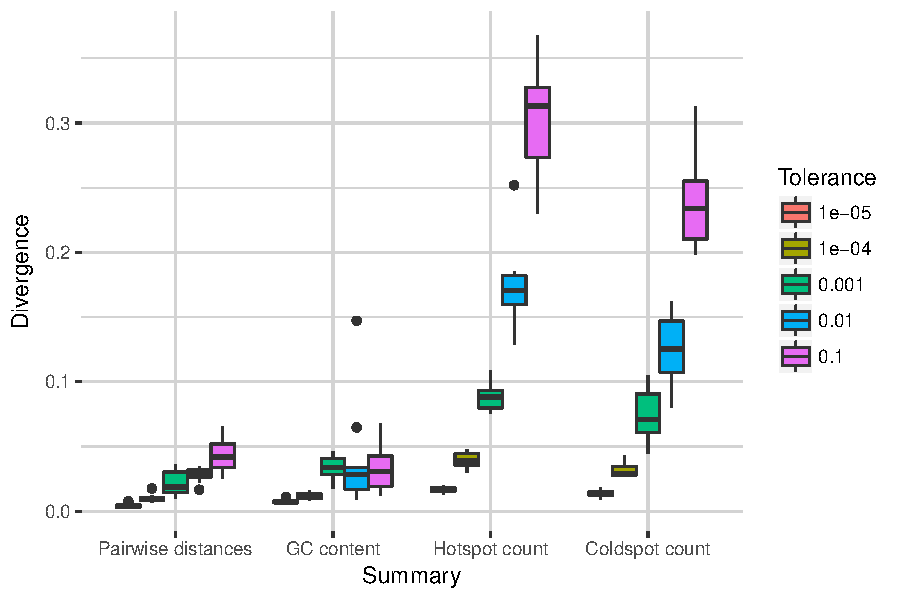
\includegraphics[width=\linewidth]{Figures/Multiple/div_by_summary_and_tol.pdf}
    \caption{KL-divergence to true summary distributions by tolerance, taken over 10 trials of the algorithm}
    \label{fig:SummaryPerformance}
\end{figure}
It appears that the summary in question does affect the KL divergence, particular seen for the hotspot count distribution.
However, in each case the KL divergence appears to approach zero exponentially as $\varepsilon \to 0$. 

These results suggest that the user should expect a high degree of accuracy for a significantly diminished runtime for any reasonable choice of tolerance $\varepsilon$, although convergence will vary between statistics.

\subsection*{Appendix B: Performance of nearest neighbor distribution subsampling algorithm}

Now, we run Algorithm \ref{NNDistributionAveraging} on \texttt{p\_f1} subsampled without replacement to 10,000 sequences.
We compute the nearest neighbor distribution of CDR3 sequences for the full subsampled dataset, as well as using Algorithm \ref{NNDistributionAveraging} with tolerances $\varepsilon \in \left\{0.1, 0.001, \dotsc, 10^{-7} \right\}$.
We replicate this experiment for 10 trials in the same manner as detailed in Appendix A.
Figure \ref{fig:NNFreqPoly} shows a frequency polygon of the same distributions.
Figure \ref{fig:NNECDF} shows their empirical cumulative distribution functions, which reveals bias in the tail of the approximation distributions.
\begin{figure}
    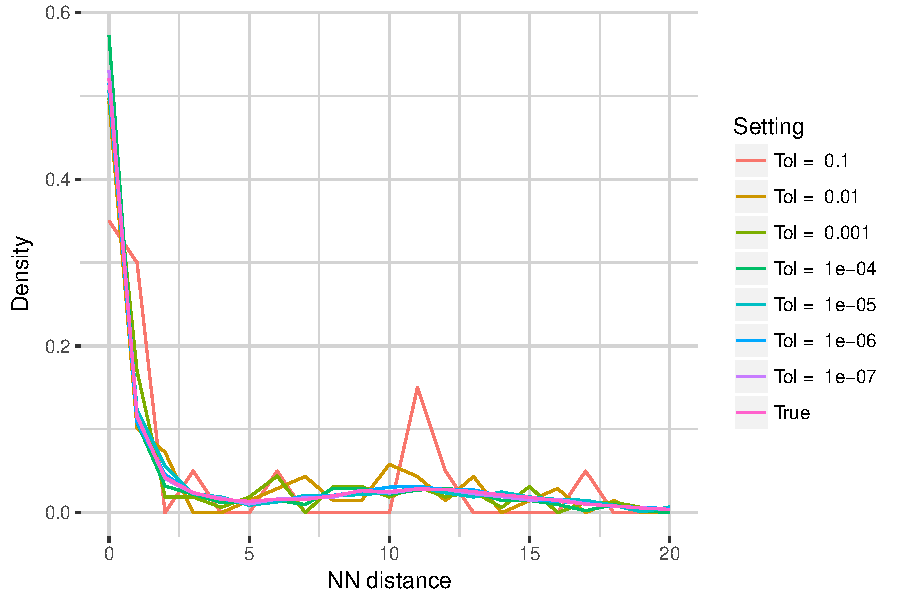
\includegraphics[width=\linewidth]{Figures/NearestNeighbor/CDR3/freqpoly_by_tol.pdf}
    \caption{Frequency polygons of true and subsampled nearest neighbor distributions by tolerance.}
    \label{fig:NNFreqPoly}
\end{figure}
\begin{figure}
    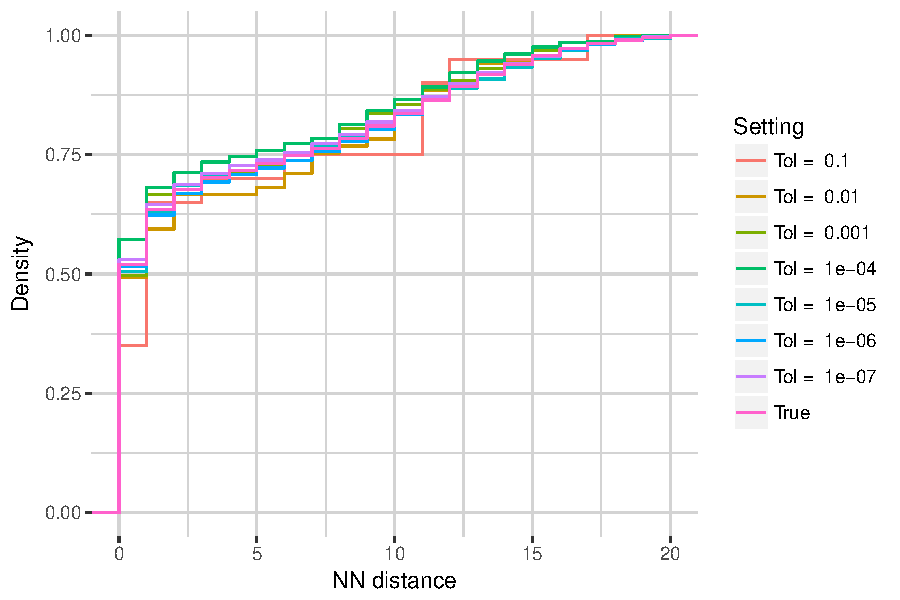
\includegraphics[width=\linewidth]{Figures/NearestNeighbor/CDR3/ecdf_by_tol.pdf}
    \caption{Empirical c.d.f. of true and subsampled nearest neighbor distributions by tolerance.}
    \label{fig:NNECDF}
\end{figure}

Figure \ref{fig:NNDivergences} displays the KL-divergence to the true distribution for each tolerance.
\begin{figure}
    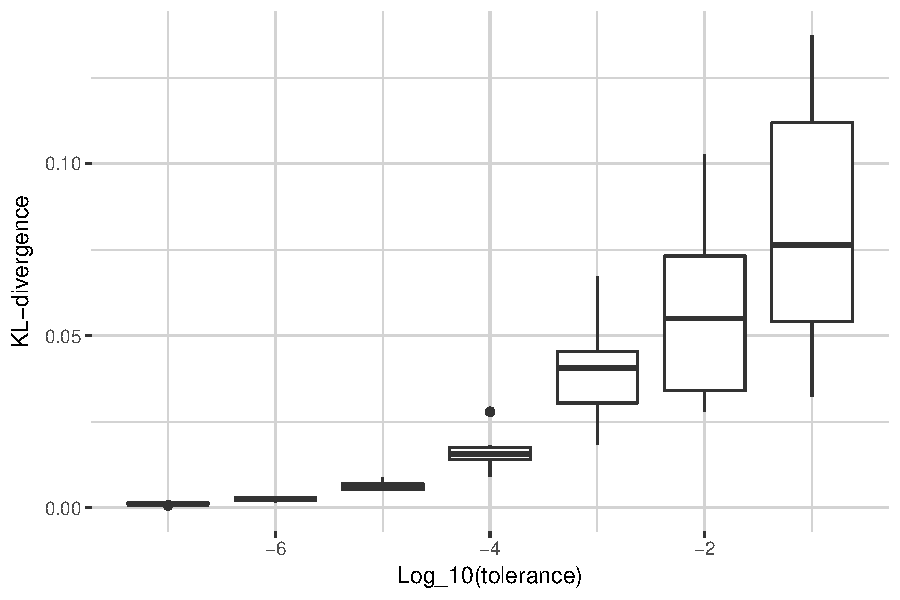
\includegraphics[width=\linewidth]{Figures/NearestNeighbor/CDR3/div_by_tol.pdf}
    \caption{KL-divergence to true nearest neighbor distribution by tolerance, taken over 10 trials of the algorithm.}
    \label{fig:NNDivergences}
\end{figure}
Figure \ref{fig:NNTimes} displays the runtimes and log-runtimes for each tolerance as well as the true "population" runtime for the full dataset.
\begin{figure}
    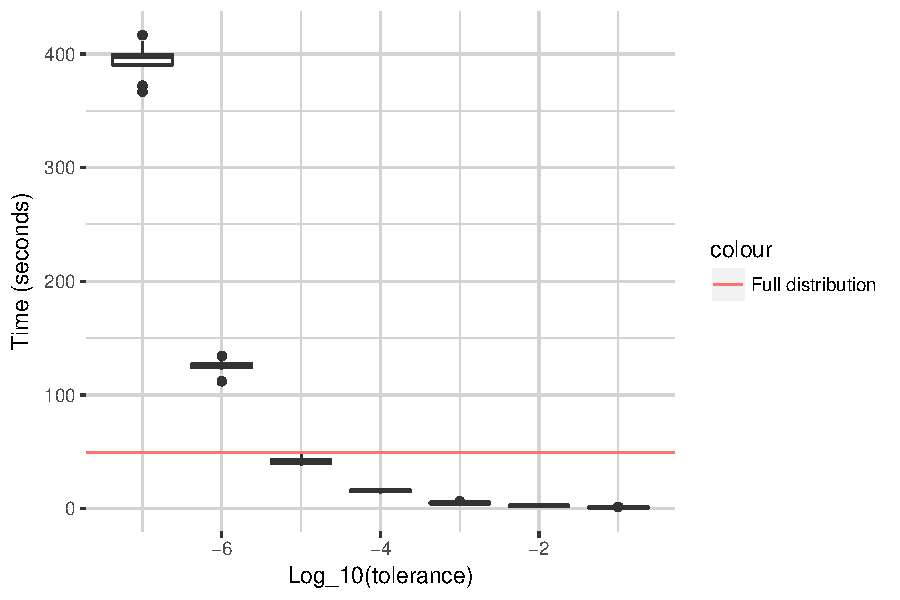
\includegraphics[width=0.9\linewidth]{Figures/NearestNeighbor/CDR3/time_by_tol.pdf}
    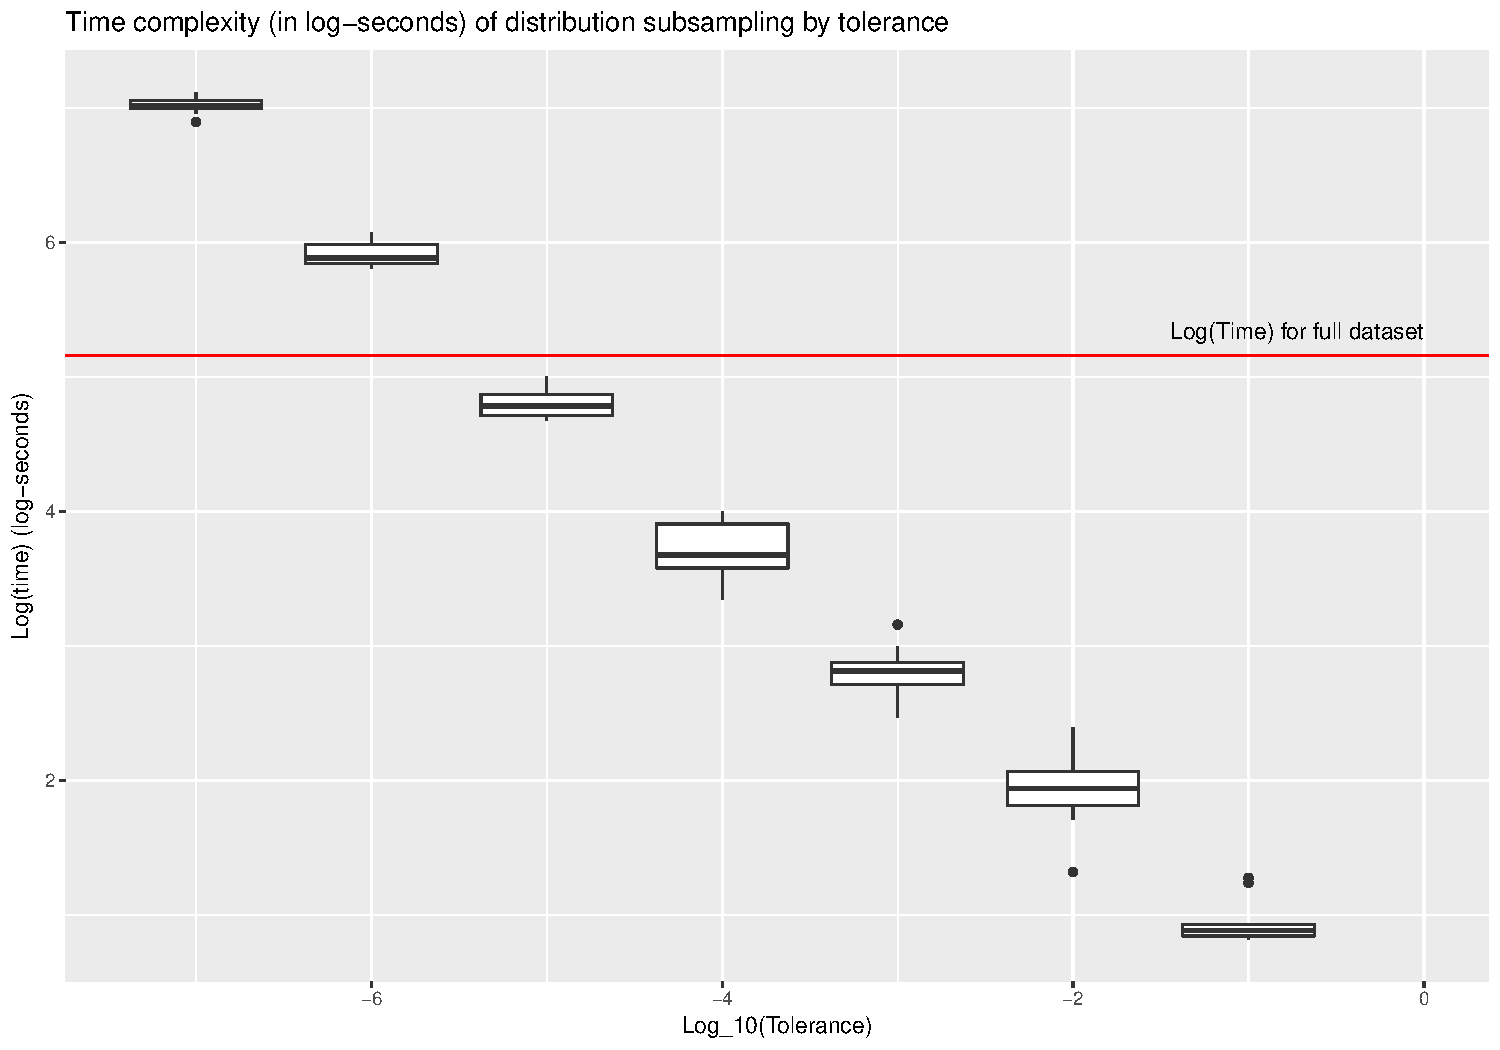
\includegraphics[width=0.9\linewidth]{Figures/NearestNeighbor/CDR3/log_time_by_tol.pdf}
    \caption{Runtime (in seconds) and log-runtime (in log-seconds) for Algorithm \ref{DistributionAveraging} by tolerance, taken over 10 trials.}
    \label{fig:NNTimes}
\end{figure}

To assess the effect of sequence lengths on Algorithm \ref{NNDistributionAveraging}, we perform the same experiment as above on query sequence reads rather than inferred CDR3 sequences.
These length distributions are different by about an order of magnitude, as seen in the table below.
\begin{figure} 
% latex table generated in R 3.4.1 by xtable 1.8-2 package
% Mon Dec 24 09:20:46 2018
\begin{tabular}{rrrrrr}
 Min. & 1st Qu. & Median & Mean & 3rd Qu. & Max. \\ 
  \hline
\hline
21 & 42 & 51 & 50.8 & 60 & 105 \\ 
  163 & 494 & 515 & 497.0 & 529 & 571 \\ 
  \end{tabular}
\label{}
\end{figure} 
.
We note that the \texttt{sequence} column is the default for Algorithm \ref{NNDistributionAveraging} within \texttt{sumrep}, although we expect users to examine this distribution for a variety of sequence types including CDR3s.
We run Algorithm \ref{NNDistributionAveraging} on the same subsampled 10,000 sequences of \texttt{p\_f1}.
We compute the nearest neighbor distribution of query sequences for the full subsampled dataset, as well as using Algorithm \ref{NNDistributionAveraging} with tolerances $\varepsilon \in \left\{0.1, 0.001, \dotsc, 10^{-5} \right\}$.
We replicate this experiment for 10 trials in the same manner as detailed in Appendix A.
Figure \ref{fig:NNFreqPolySequence} shows a frequency polygon of the same distributions.
Figure \ref{fig:NNECDFSequence} shows their empirical cumulative distribution functions, which reveals bias in the tail of the approximation distributions.
\begin{figure}
    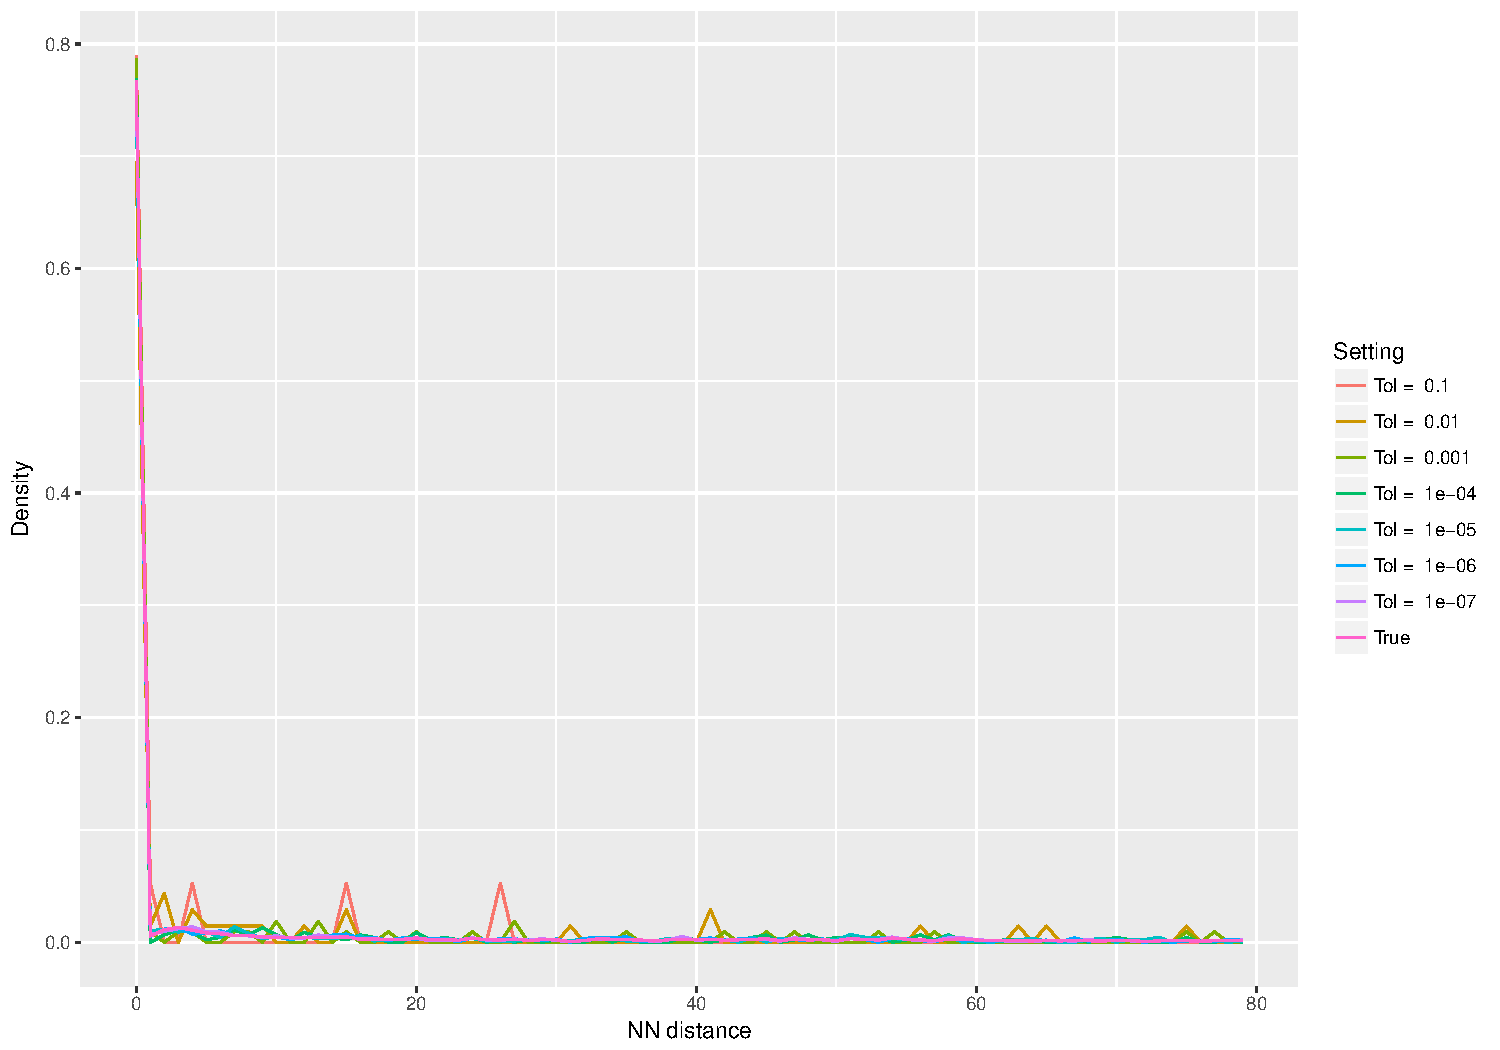
\includegraphics[width=\linewidth]{Figures/NearestNeighbor/Sequence/freqpoly_by_tol.pdf}
    \caption{Frequency polygons of true and subsampled nearest neighbor distributions by tolerance.}
    \label{fig:NNFreqPolySequence}
\end{figure}
\begin{figure}
    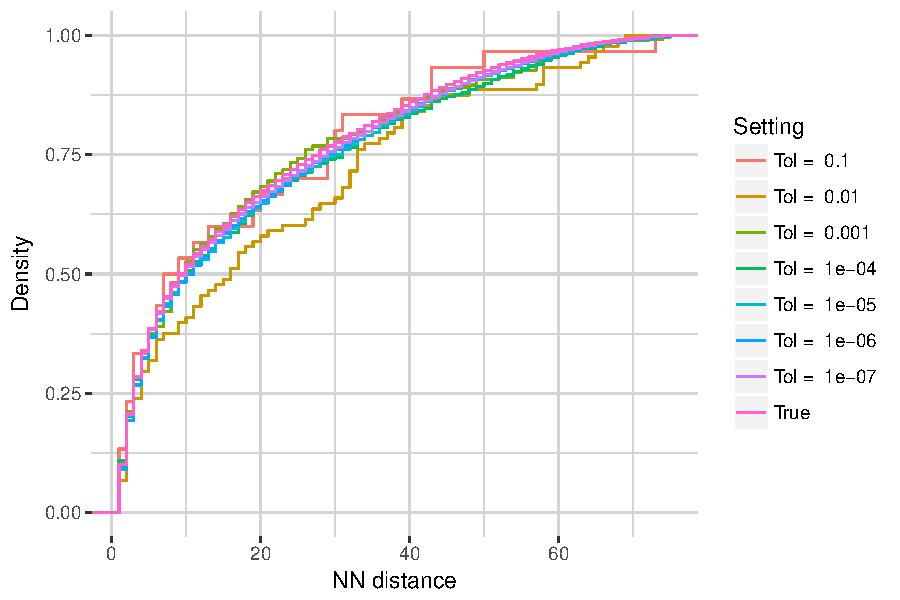
\includegraphics[width=\linewidth]{Figures/NearestNeighbor/Sequence/ecdf_by_tol.pdf}
    \caption{Empirical c.d.f. of true and subsampled nearest neighbor distributions by tolerance.}
    \label{fig:NNECDFSequence}
\end{figure}

Figure \ref{fig:NNDivergencesSequence} displays the KL-divergence to the true distribution for each tolerance.
\begin{figure}
    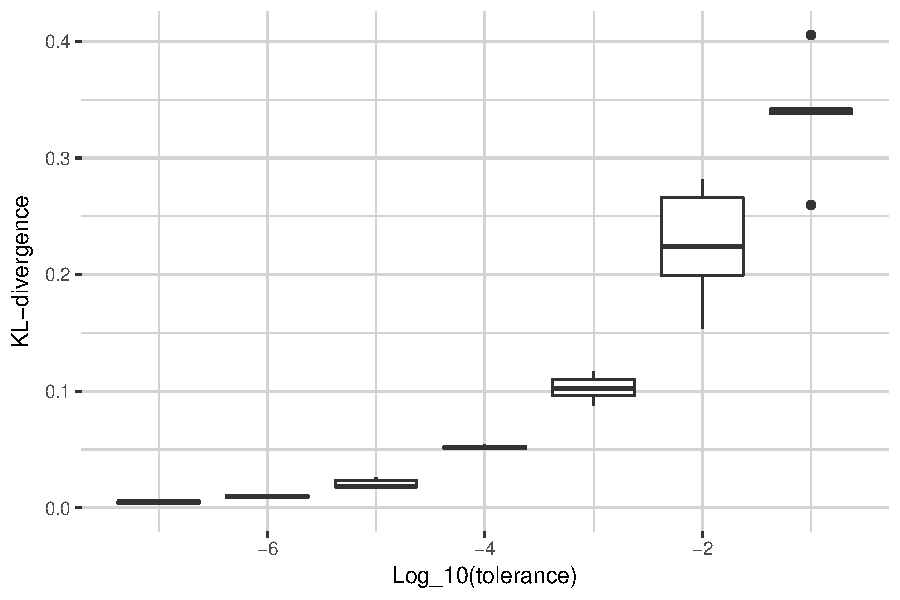
\includegraphics[width=\linewidth]{Figures/NearestNeighbor/Sequence/div_by_tol.pdf}
    \caption{KL-divergence to true nearest neighbor distribution by tolerance, taken over 10 trials of the algorithm.}
    \label{fig:NNDivergencesSequence}
\end{figure}
Figure \ref{fig:NNTimesSequence} displays the runtimes and log-runtimes for each tolerance as well as the true "population" runtime for the full dataset.
\begin{figure}
    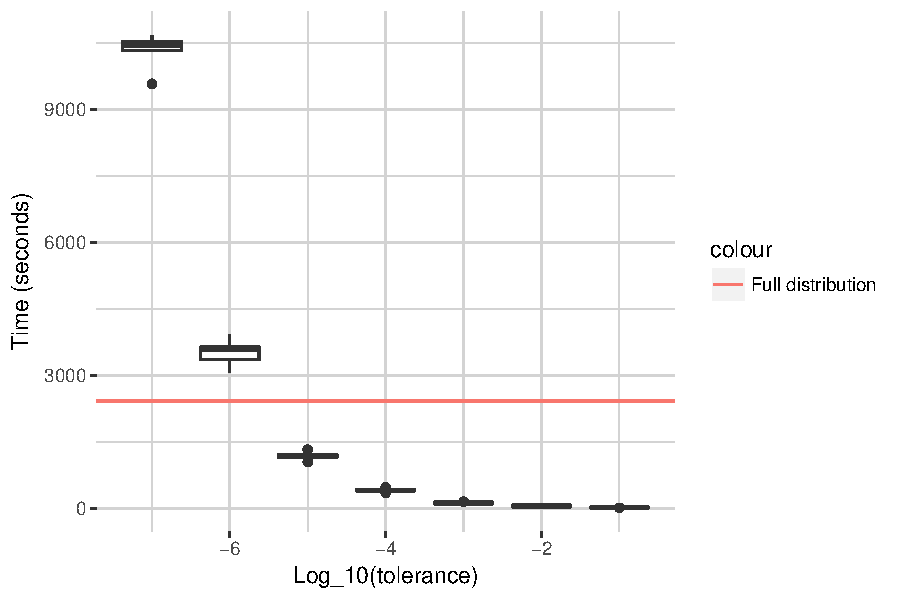
\includegraphics[width=0.9\linewidth]{Figures/NearestNeighbor/Sequence/time_by_tol.pdf}
    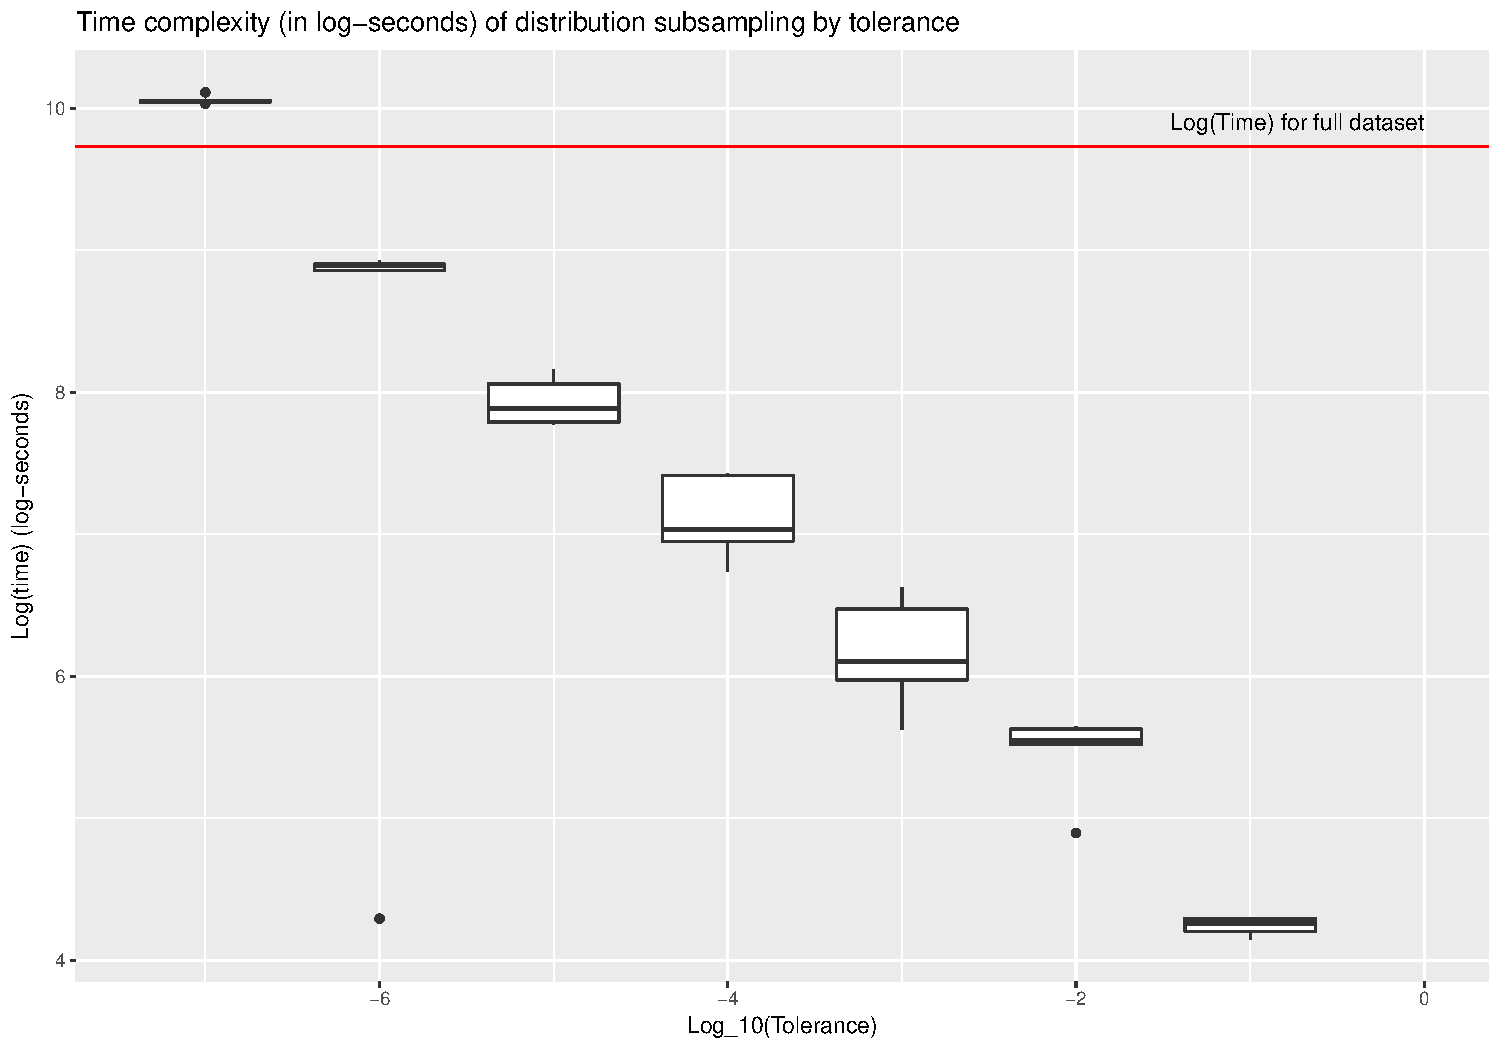
\includegraphics[width=0.9\linewidth]{Figures/NearestNeighbor/Sequence/log_time_by_tol.pdf}
    \caption{Runtime (in seconds) and log-runtime (in log-seconds) for Algorithm \ref{DistributionAveraging} by tolerance, taken over 10 trials.}
    \label{fig:NNTimesSequence}
\end{figure}
Overall, Algorithm \ref{NNDistributionAveraging} has more trouble honing in on the nearest neighbor distribution of query sequences as quickly as it does for CDR3s, although the runtime efficiency appears to be higher.
This is likely due to the pecularities of the full NN distribution of query sequences, in which roughly 75\% of the mass is at zero and the remaning 25\% is gradually and nonuniformly dispersed over the values 1 through about 80.
Nonetheless, the approximate distributions appear to converge to the truth as $\varepsilon \to 0$, and the stastical characteristics of the full distribution are captured for even small values of $\varepsilon$.


Next we investigate the effect of dataset size on the performance of Algorithm \ref{NNDistributionAveraging}.
For sample sizes $s \in \{\exp(6), \dots, \exp(10)\}$, we subsample \texttt{p\_f1} without replacement to $s$ sequences and compute the pairwise distance distribution of CDR3 sequences for the full subsampled dataset as well as those given by tolerances $\varepsilon \in \{0.1, ..., 10^{-5}\}$.  
We perform this experiment 5 times for each $s$.
Boxplots of the KL-divergence by log(size) and tolerance over all trials are displayed in Figure \ref{fig:DivBySize}.  
\begin{figure}
    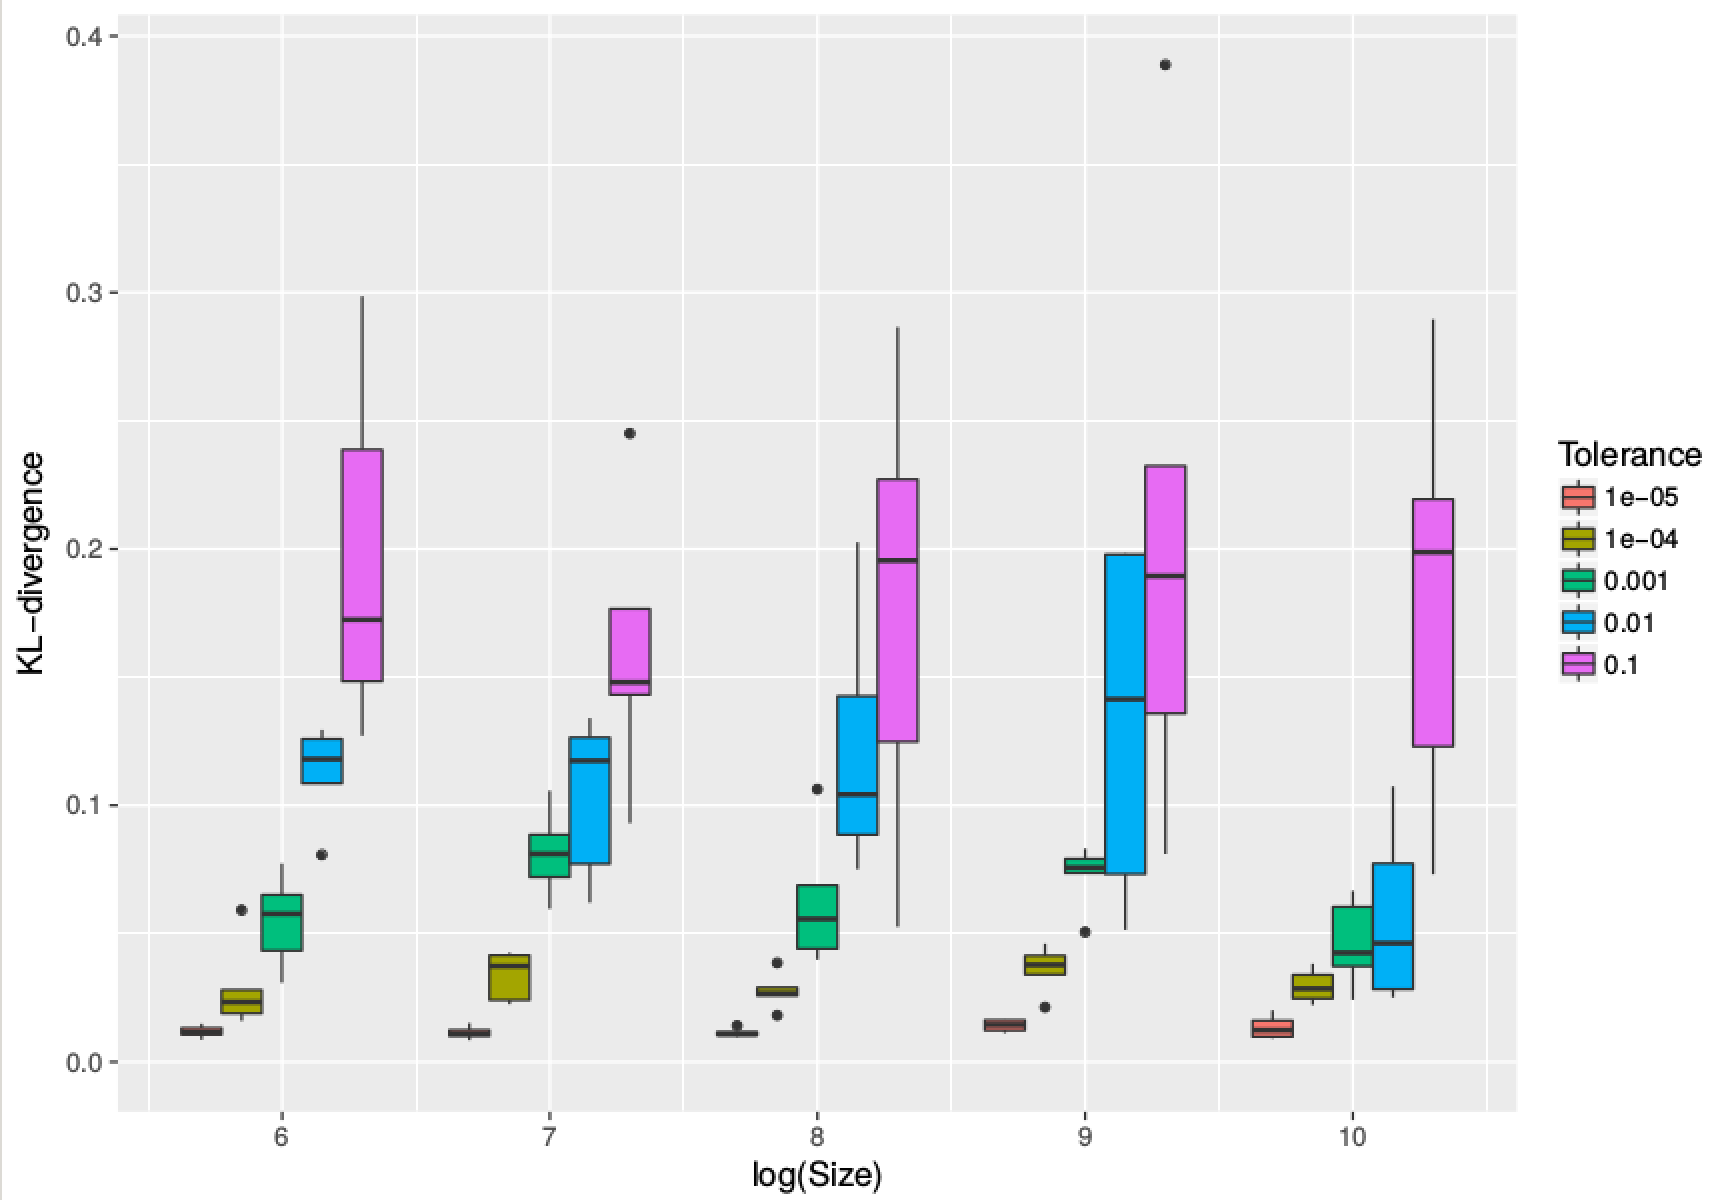
\includegraphics[width=\linewidth]{Figures/NearestNeighbor/div_by_size_and_tol_cdr3.png}
    \caption{KL-divergence to true nearest neighbor distribution by tolerance and log(size) of dataset, taken over 10 trials of the algorithm.}
    \label{fig:DivBySize}
\end{figure}
There is not an apparent trend of the KL-divergence that is consistent across tolerances, although there is much higher variation for higher tolerances than lower ones.
Figure \ref{fig:TimeBySize} shows boxplots of the runtime of the procedure for each scenario.
\begin{figure}
    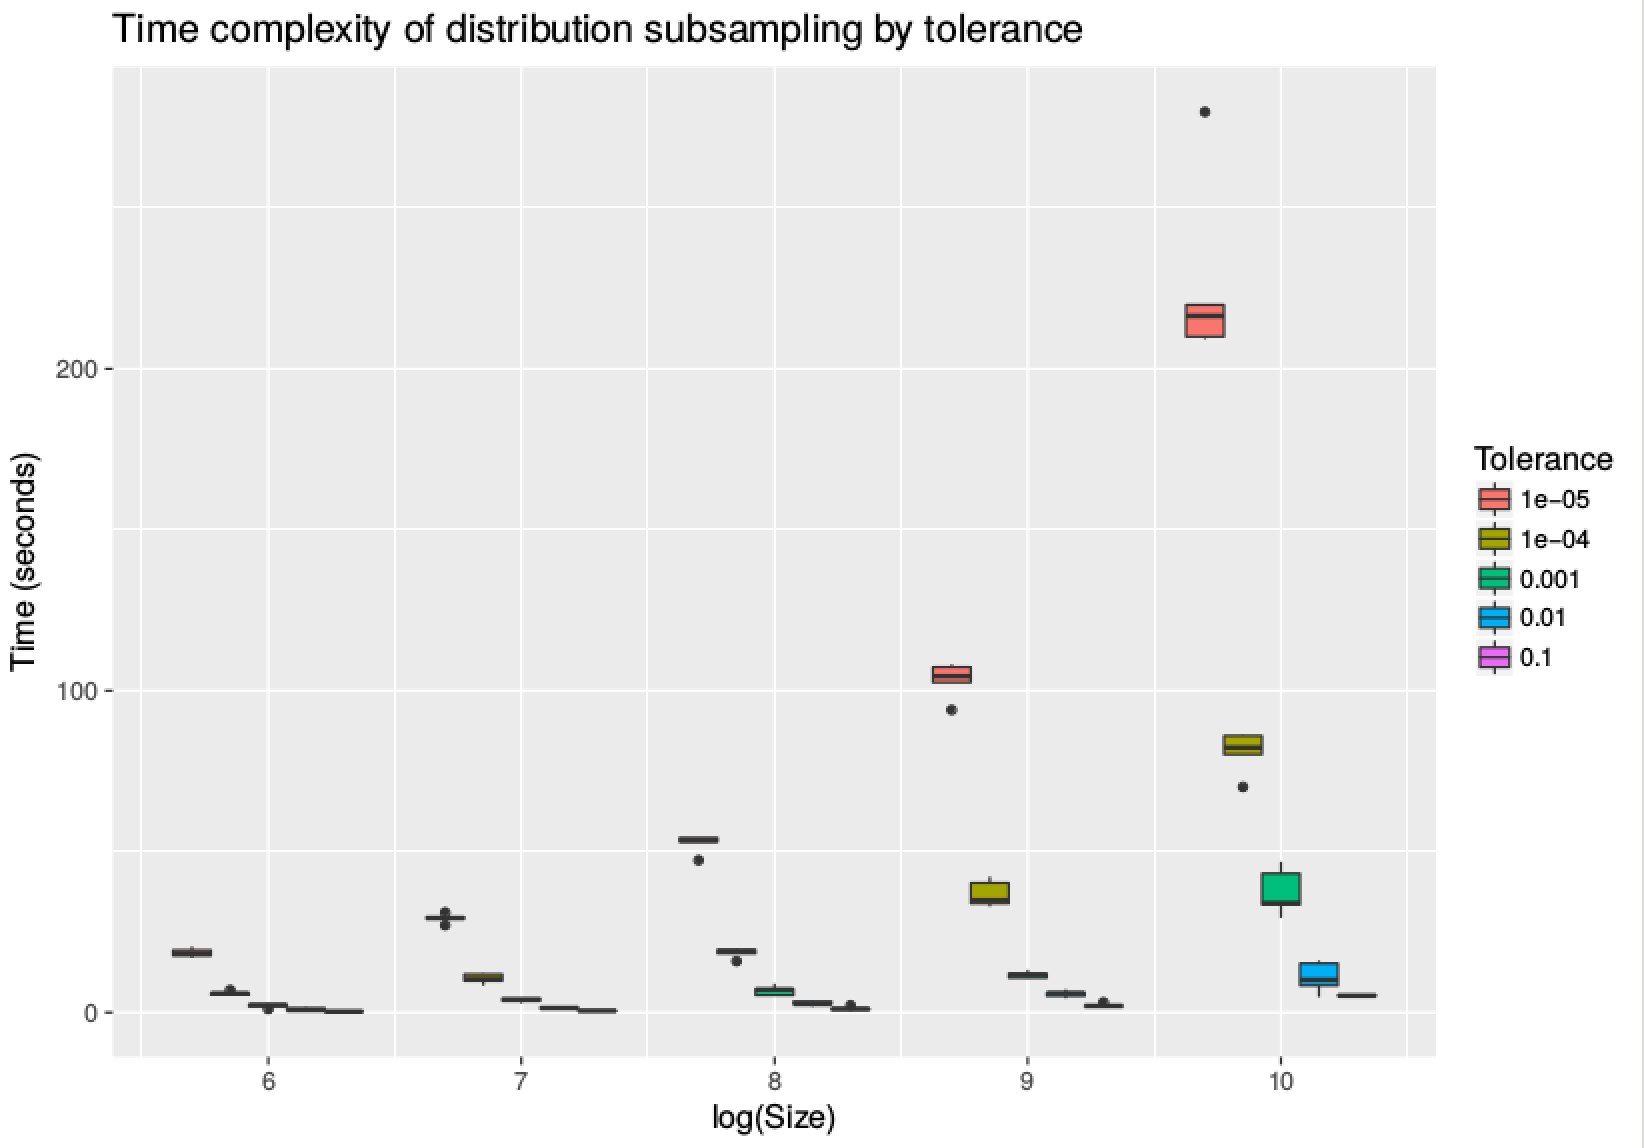
\includegraphics[width=\linewidth]{Figures/NearestNeighbor/time_by_size_and_tol_cdr3.png}
    \caption{KL-divergence to true nearest neighbor distribution by tolerance and log(size) of dataset, taken over 10 trials of the algorithm.}
    \label{fig:TimeBySize}
\end{figure}
As expected, runtime increases as tolerance decreases, but also increases with the size of the dataset which deviates from the behavior of Algorithm \ref{DistributionAveraging}, where dataset size did not seem to affect runtime.
This is reasonable since each batch iteration of \ref{NNDistributionAveraging} must compute the nearest neighbor distance from each sequence in batch $B$ to the full repertoire $R$, which is $\mathcal O(n^2 m)$, where $n = \text{card}(R)$ is the number of sequences in the full repertoire, and $m = \max_{s \in B} \text{length}(s)$ is the largest sequence length in the batch sample.

To get a better picture of what is happening, we can also look at the time efficiency for each case, defined to be 
\begin{align}
    \text{Efficiency} := \frac{\text{time to compute full distribution}}{\text{time to compute approximate distribution}}
\end{align}
where the denominator of course depends on the size of the dataset and tolerance $\varepsilon$.
This is shown in Figure \ref{fig:EfficiencyBySize}.
\begin{figure}
    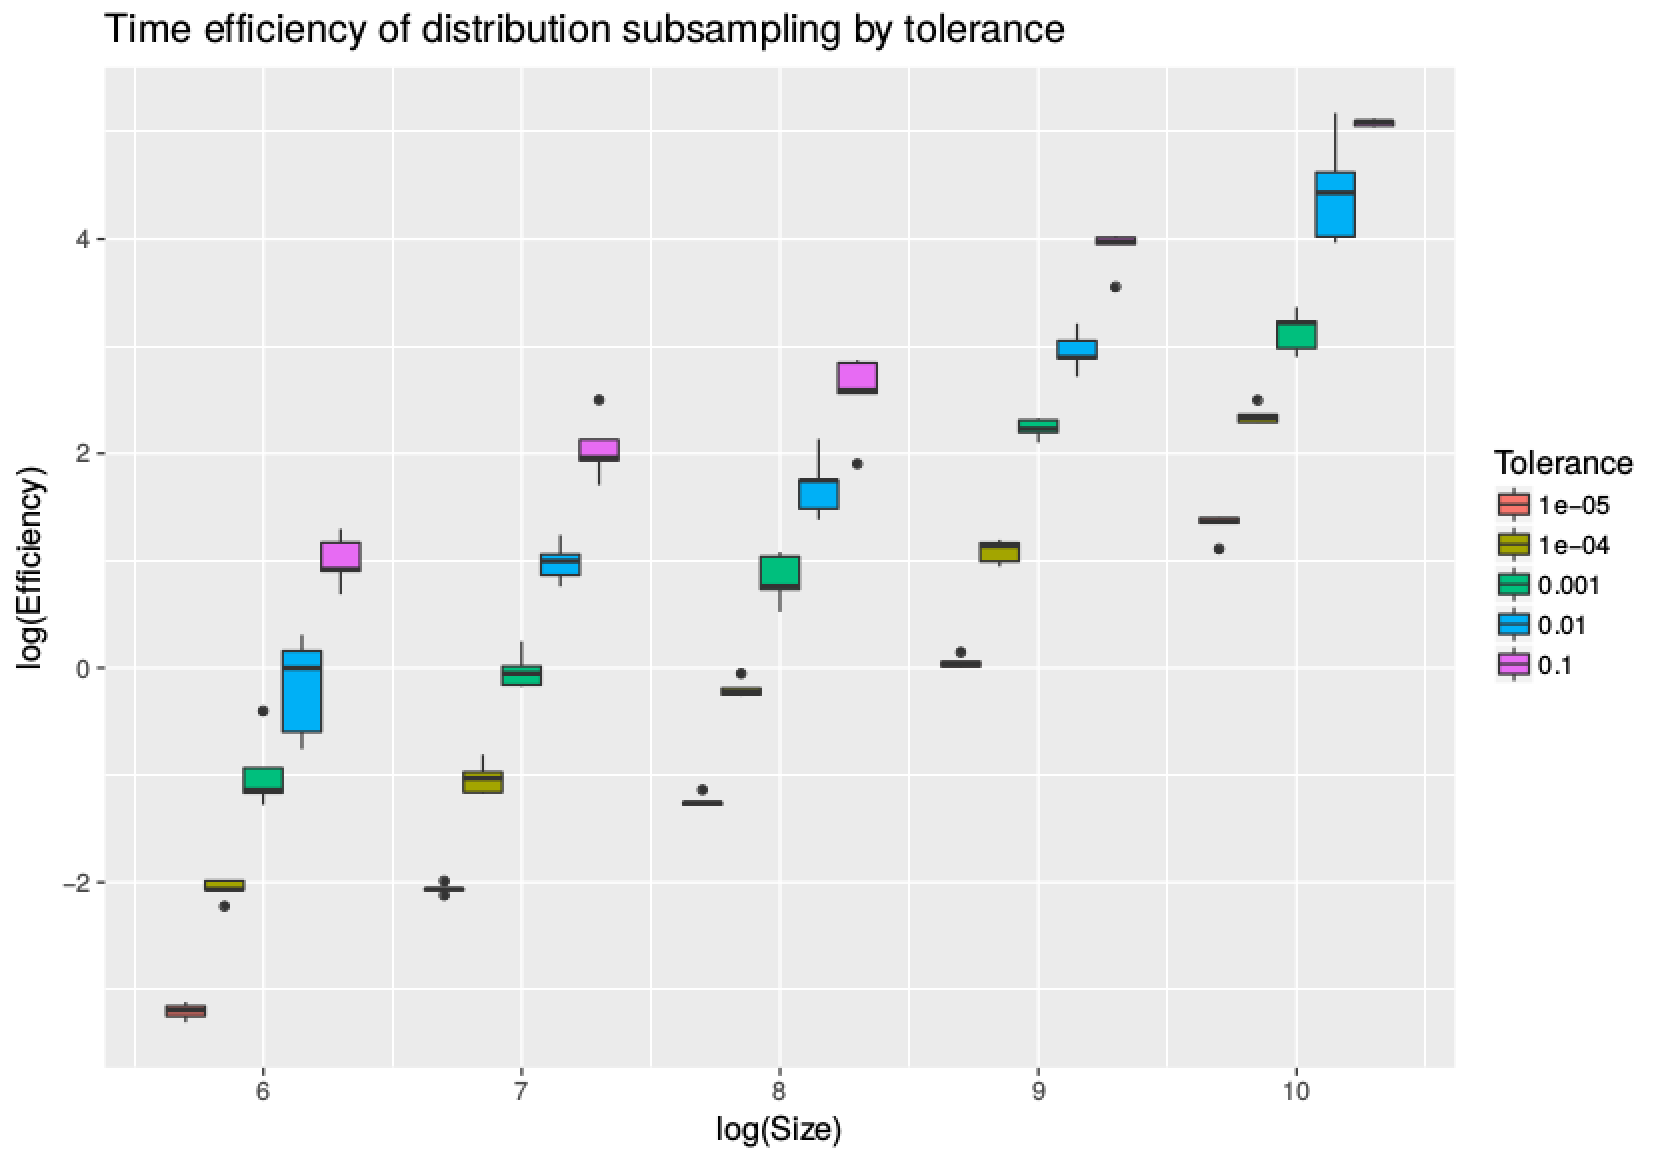
\includegraphics[width=\linewidth]{Figures/NearestNeighbor/efficiency_by_size_and_tol_cdr3.png}
    \caption{KL-divergence to true nearest neighbor distribution by tolerance and log(size) of dataset, taken over 10 trials of the algorithm.}
    \label{fig:EfficiencyBySize}
\end{figure}
Note the log-log scale, so that the line $y=0$ corresponds to instances when the true and approximate routines have identical runtimes.
Thus, the region $y > 0$ corresponds to instances when Algorithm \ref{NNDistributionAveraging} outperforms the computation of the full nearest neighbor distribution.
We see that efficiency increases with dataset size as well as tolerance.
The former verifies that the complexity of the approximation routine is lower than that of computing the full distirbution.
Examining the boxplots near $y = 0$ by $\log(\text{size})$, we see that for a dataset of size $\exp(k)$, we would need a tolerance of at least $\frac{1}{10^{k - 4}}$.
For example, for $\log(\text{size}) = 6$, we see that tolerances higher than $0.01 = \frac{1}{100} = \frac{1}{10^{6 - 4}}$ would on average yield an efficiency greater than one.
This suggests that, for a dataset with $n$ CDR3 sequences, a sensible rule of thumb would be to choose $\varepsilon > \frac{1}{10^{k - 4}} = \frac{1}{10^{\log(n) - 4}}$.
This will of course be more or less appropriate for a given dataset depending on the nature of the repertoire from which it was sampled.

Next, we compute the pairwise distance distribution of full query sequence reads, using the same settings as before.
Figures \ref{fig:DivBySizeFull}, \ref{fig:TimeBySizeFull}, and \ref{fig:EfficiencyBySizeFull} display boxplots of the KL-divergence to truth, runtime, and time efficiency, respectively.
\begin{figure}
    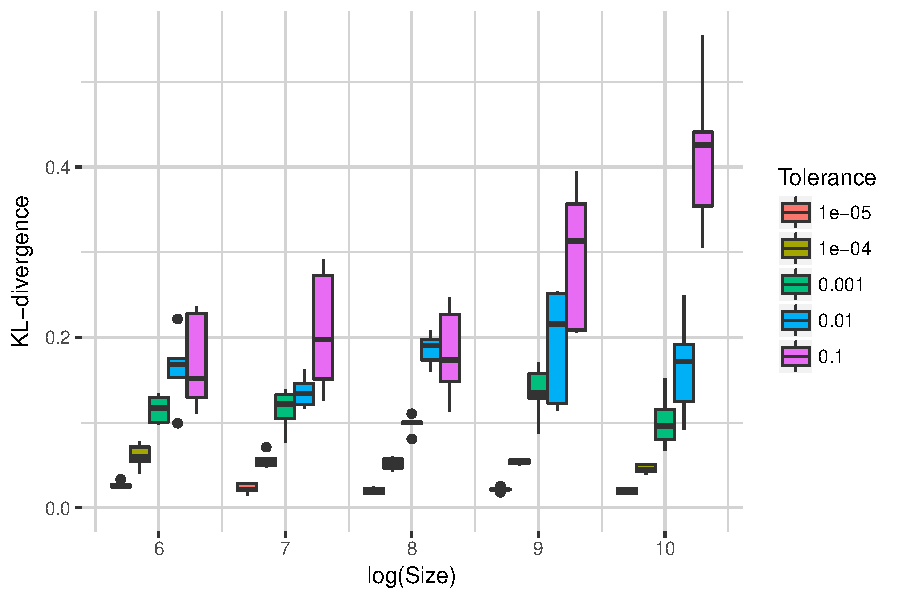
\includegraphics[width=\linewidth]{Figures/NearestNeighbor/div_by_size_and_tol.pdf}
    \caption{KL-divergence to true nearest neighbor distribution by tolerance and log(size) of dataset, taken over 10 trials of the algorithm.}
    \label{fig:DivBySizeFull}
\end{figure}
\begin{figure}
    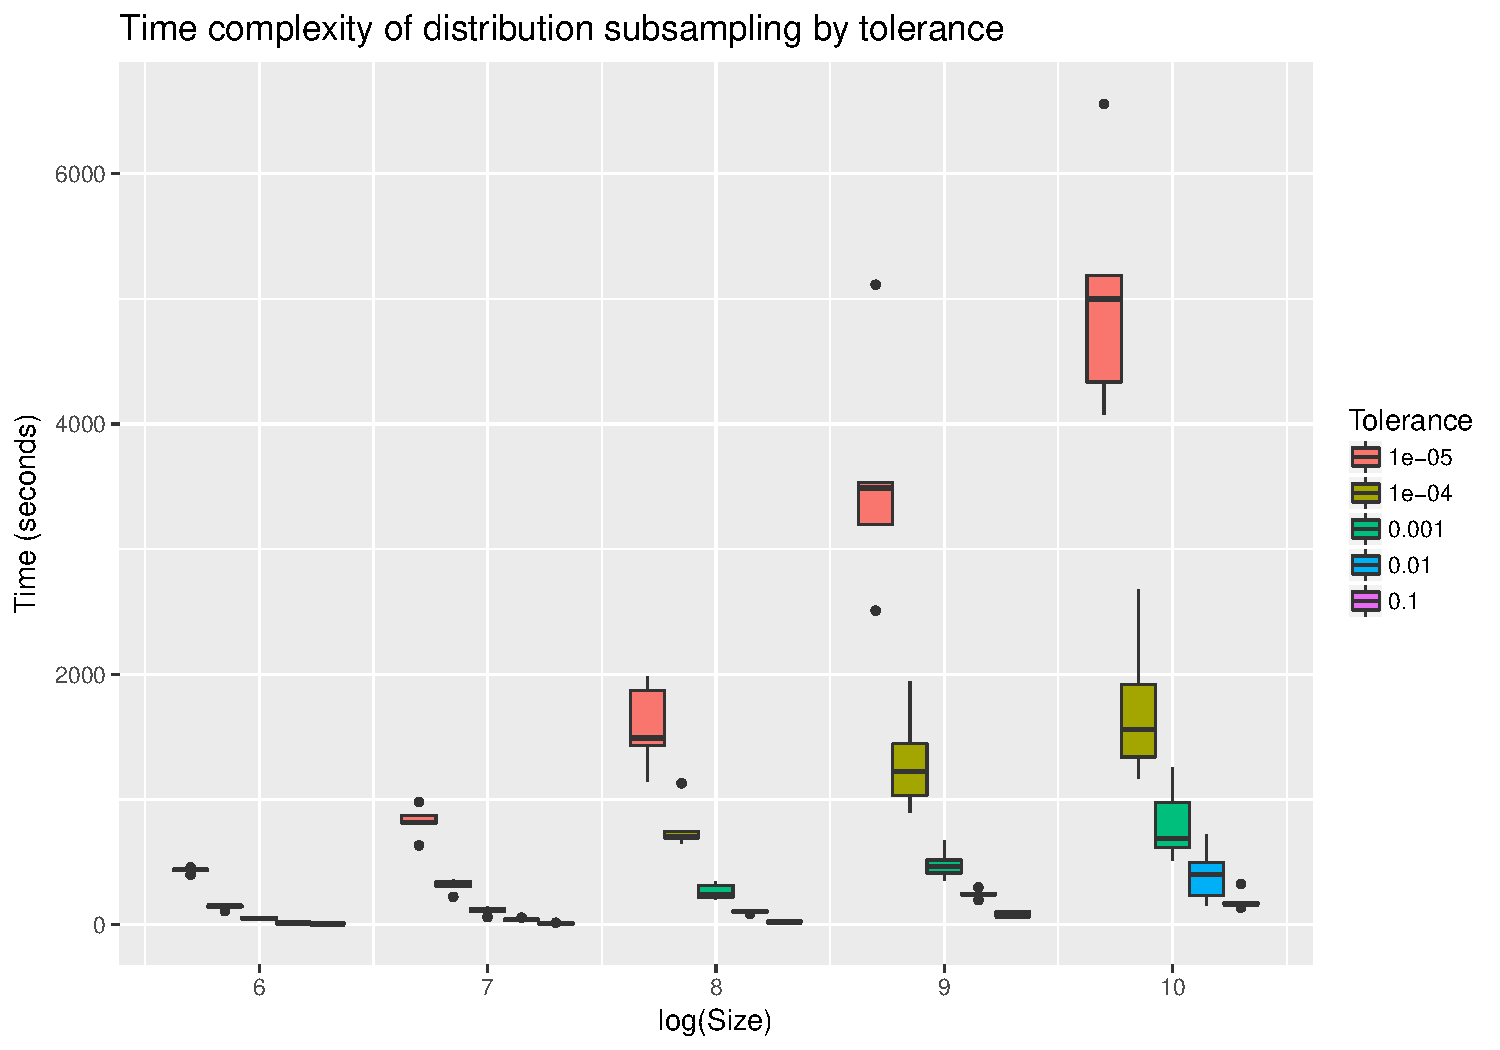
\includegraphics[width=\linewidth]{Figures/NearestNeighbor/time_by_size_and_tol.pdf}
    \caption{KL-divergence to true nearest neighbor distribution by tolerance and log(size) of dataset, taken over 10 trials of the algorithm.}
    \label{fig:TimeBySizeFull}
\end{figure}
\begin{figure}
    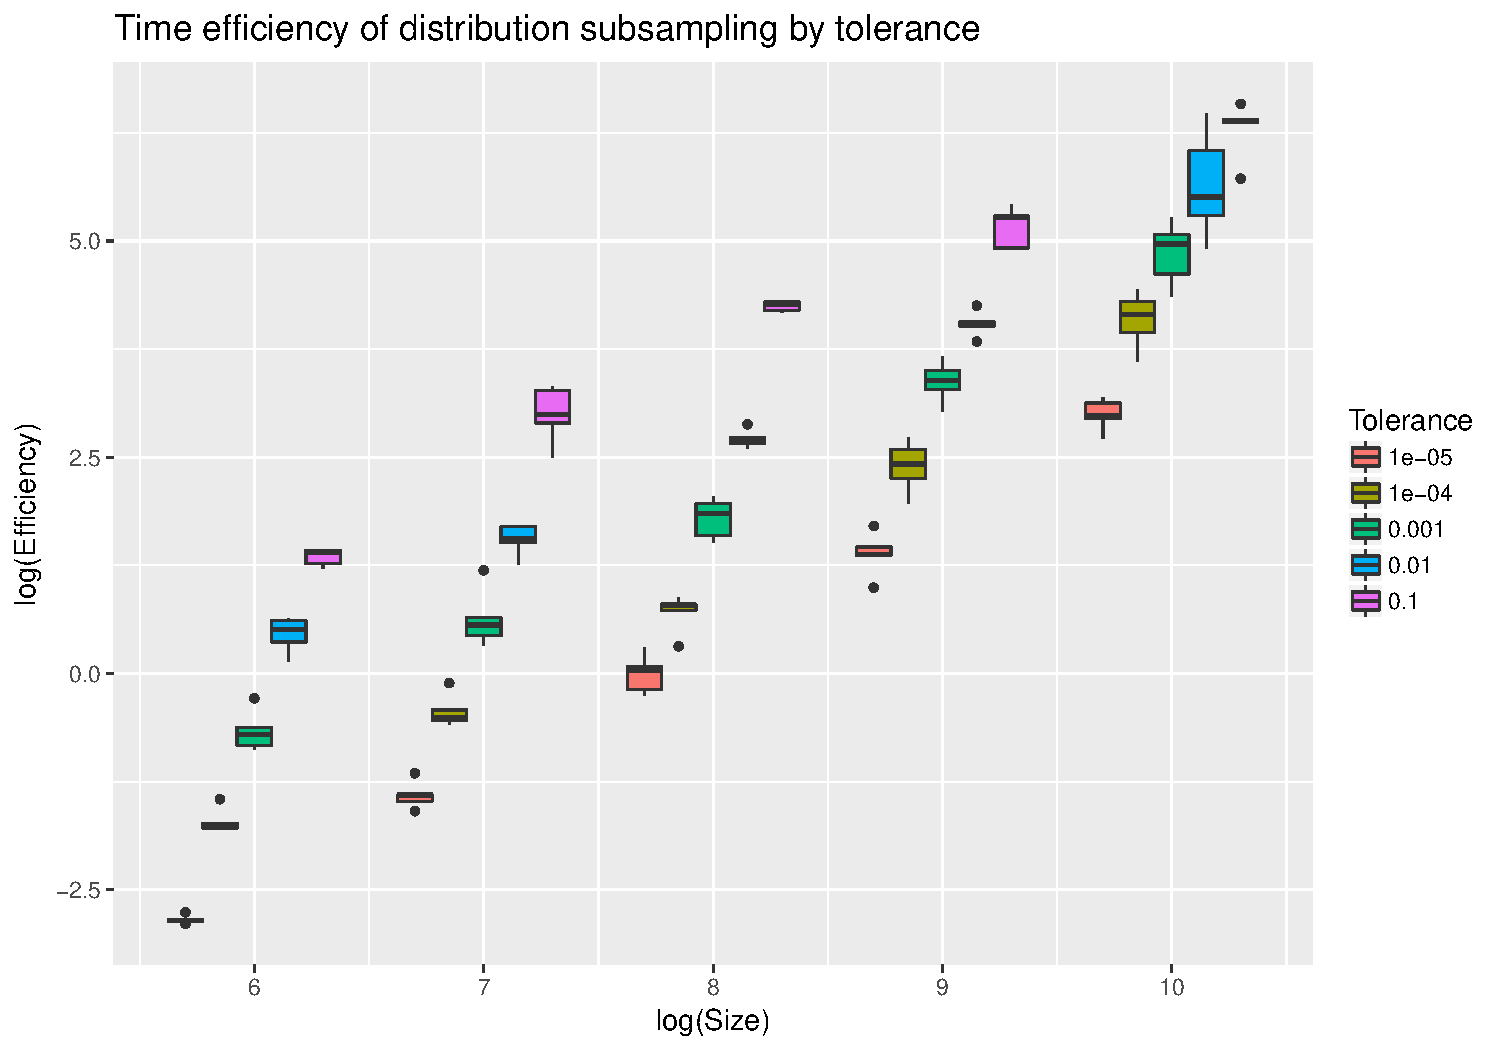
\includegraphics[width=\linewidth]{Figures/NearestNeighbor/efficiency_by_size_and_tol.pdf}
    \caption{KL-divergence to true nearest neighbor distribution by tolerance and log(size) of dataset, taken over 10 trials of the algorithm.}
    \label{fig:EfficiencyBySizeFull}
\end{figure}
We see similar patterns as before, although numerical ranges differ when looking at query sequences versus CDR3 sequences.
For example, the KL-divergences are consistently higher for each (tolerance, sample size) scenario, although they still seem to decay towards zero.
This is likely due to the fact that raw sequence reads exhibit significantly more noise than CDR3 sequences.
%BJO ^ This is an educated guess, since query sequences can in principle take many arbitrary forms, whereas CDR3 inferences are necessarily multiples of 3, and heavily constrainted by the inferred naive sequence
Moreover, the runtime by dataset size is consistently higher, with runtimes of over an hour for datasets of size $\exp(10) \approx 22,000$ sequences and a tolerance of $10^{-5}$. 
Still, as evidenced by Figure \ref{fig:EfficiencyBySizeFull}, these runtimes are consistently at least $\exp(2.5) \approx 12$ times smaller than computing the full distribution, with efficiencies as high as $\exp(6.25) \approx 457$ for datasets of size $\exp(10)$.
While there is a tradeoff between minimizing the KL-divergence to truth and maximizing the time efficiency when choosing the tolerance, these results suggest that any reasonable choice of tolerance will outperform computing the full distribution for moderate and large datasets.
The user should use these results as well as problem-specific considerations when deciding whether or not to use Algorithm \ref{NNDistributionAveraging} instead of computing the full distribution, and if so, which tolerance to use.

\end{document}
